\documentclass[9pt]{beamer}
\usepackage[utf8]{inputenc}
\usepackage[T1]{fontenc}
\usepackage[utf8]{inputenc}
%!TEX encoding = UTF-8 Unicode
\usefonttheme[onlymath]{serif}
\usepackage{listings}
\usepackage{caption}  
\usepackage{hyperref}
\hypersetup{
    %colorlinks=true,
    %linkcolor=blue,
    %filecolor=magenta,      
    urlcolor=blue,
}
\urlstyle{same}
\usepackage{multicol}
\usepackage{graphics}
\usepackage{multimedia}
\usepackage{media9}
\usepackage{graphicx}
\usepackage{empheq}
\usepackage{color}
\usepackage{siunitx}
\usepackage[many]{tcolorbox}
\tcbset{highlight math style={enhanced,
  colframe=red,colback=white,arc=0pt,boxrule=1pt}}
  \tcbset{highlight math style={enhanced,
  colframe=red!60!black,colback=yellow!50!white,arc=4pt,boxrule=1pt,
  drop fuzzy shadow}}
\usepackage{verbatim}
\usepackage{listings}
\usepackage{xcolor}
\definecolor{mygray}{RGB}{245,245,245}
\definecolor{ipython_bg}{RGB}{247, 247, 247}
\definecolor{comentaryGreen}{rgb}{0,0.6,0}
\lstset{
  language=Python,
  numbers=left,
  numberstyle=\footnotesize,
  stepnumber=1,
  columns=fullflexible,
  showspaces=false,
  showstringspaces=false,
  showtabs=false,
  frame=single,
  framerule=0pt,
  basicstyle           = {\normalsize\ttfamily},
  keywordstyle      = \color{blue},
  commentstyle=\color{comentaryGreen},
  stringstyle           = \color{red},
  numberstyle       = \scriptsize\color{gray},
  breaklines=false,
  breakatwhitespace=false,
  escapeinside={\%*}{*)}
}
\usepackage[utf8]{inputenc}

\usetheme{Warsaw}

%Information to be included in the title page:
\title{Radioprotezione nello Spazio}
\subtitle[]{Dosimetria}
%\author[]{Lorenzo Marini \\   
%le parentesi quadre \author{Lorenzo Marini} servono a rimuovere il nome dalla barra in basso a sinistra.
%\small \texttt{lorenzo.marini.1996@gmail.com}}
\author{Lorenzo Marini} 
\institute{Dipartimento di Fisica, Pisa}
\date[Luglio 2020] % (optional)
{Esame, Luglio 2020}

\setbeamertemplate{section in toc}{\hspace*{1em}\inserttocsectionnumber.~\inserttocsection\par}
\setbeamertemplate{subsection in toc}{\hspace*{2em}\inserttocsectionnumber.\inserttocsubsectionnumber.~\inserttocsubsection\par}

\begin{document}

\setbeamertemplate{page number in head/foot}[totalframenumber] 
%%%%%%%%%%%%%%%%%%%%%%%%%%%%%%%%%%%%%%%%%%%%%

\frame{\titlepage}


%==================================================================
						%SLIDE - \tableofcontents
%==================================================================

\begin{frame} 
  	\tableofcontents
\end{frame}

%==================================================================
						%SLIDE - Introduzione
%==================================================================

\begin{frame} [fragile]
	\frametitle{Introduzione}
	
Il nostro pianeta \`e costantemente bombardato da \textcolor{blue}{raggi cosmici galattici} presenti  nello spazio interstellare.
\newline

Rappresentano un enorme  \textcolor{blue}{ostacolo alle missioni spaziali}.
\newline
 
Possono causare il \textcolor{blue}{cancro} e altri problemi di salute negli astronauti esposti. 
\newline

Non abbiamo ancora metodi efficaci per proteggere i veicoli spaziali e i loro occupanti con sufficiente sicurezza.
 \newline
 
Le agenzie spaziali (\textcolor{red}{ESA}\footnote{European Space Agency}, \textcolor{red}{NASA}\footnote{National Aeronautics and Space Administration (USA)}) hanno promosso programmi di ricerca negli ultimi 20 anni per  \textcolor{blue}{quantificare i rischi associati all'esposizione alle radiazioni nello spazio e sviluppare contromisure}. 

\end{frame}
	
%==================================================================
				%SLIDE - Introduzione - Rischi Principali
%==================================================================

\begin{frame} [fragile]
	\frametitle{Introduzione - Rischi Principali}
	\begin{minipage}{1\textwidth}
	  \begin{figure}
	  \centering
			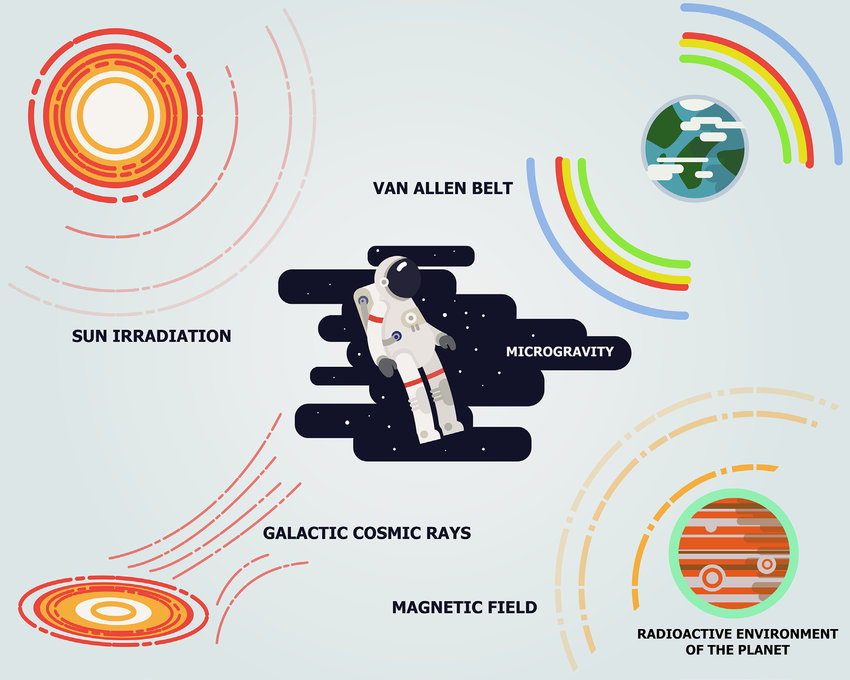
\includegraphics[scale=0.2]{figures/fig3.jpeg}
			%\caption{}
		\end{figure}
	\end{minipage}
	\newline
	
Tre  \textcolor{blue}{principali rischi} identificati nello spazio:
\begin{block}

\begin{enumerate}
\item Problemi fisiologici causati da \textcolor{red}{microgravit\`a} (o gravit\`a ridotta).
\item Problemi psicologici e medici causati dall' \textcolor{red}{isolamento}.
\item Rischi acuti e tardivi causati dall' \textcolor{red}{esposizione alle radiazioni}.
\end{enumerate}
\end{block}
\end{frame}
	
%==================================================================
				%SLIDE - Il campo di radiazione nello spazio
%==================================================================

\section{Il campo di radiazione nello spazio}
\begin{frame} [fragile]
\small
	\frametitle{Il campo di radiazione nello spazio}
	\begin{columns}
  \begin{column}{0.50\textwidth}
 
 \begin{block}{Fonti di radiazioni rilevanti nello spazio}
    \begin{itemize}
\item Galactic Cosmic Rays (\textcolor{blue}{GCR})
\item Solar Particle Events (\textcolor{blue}{SPE})
\item Radiazione Confinata (\textcolor{blue}{TP})
\end{itemize}
\end{block}


\begin{itemize}
\item \textcolor{blue}{Galactic Cosmic Rays}:
\begin{itemize}
\item \textcolor{red}{Spettro}:
\begin{itemize}
\item 87$\%$ protoni
\item 12$\%$ ioni $He$
\item 1$\%$ ioni pesanti
\end{itemize}
\item \textcolor{red}{Flusso}: 4 particelle/($cm^{2}$ $s$) al minimo solare
\item \textcolor{red}{Dose} $\approx$ 1 mSv/day 
\end{itemize}
\end{itemize}
%La radiazione confinata ($TP$) \`e formata da $e^{-}$ e $p$ intrappolati nel campo magnetico della Terra.
	 \end{column}
    \begin{column}{0.50\textwidth}
 %\newline
   \begin{figure}
	  \centering
			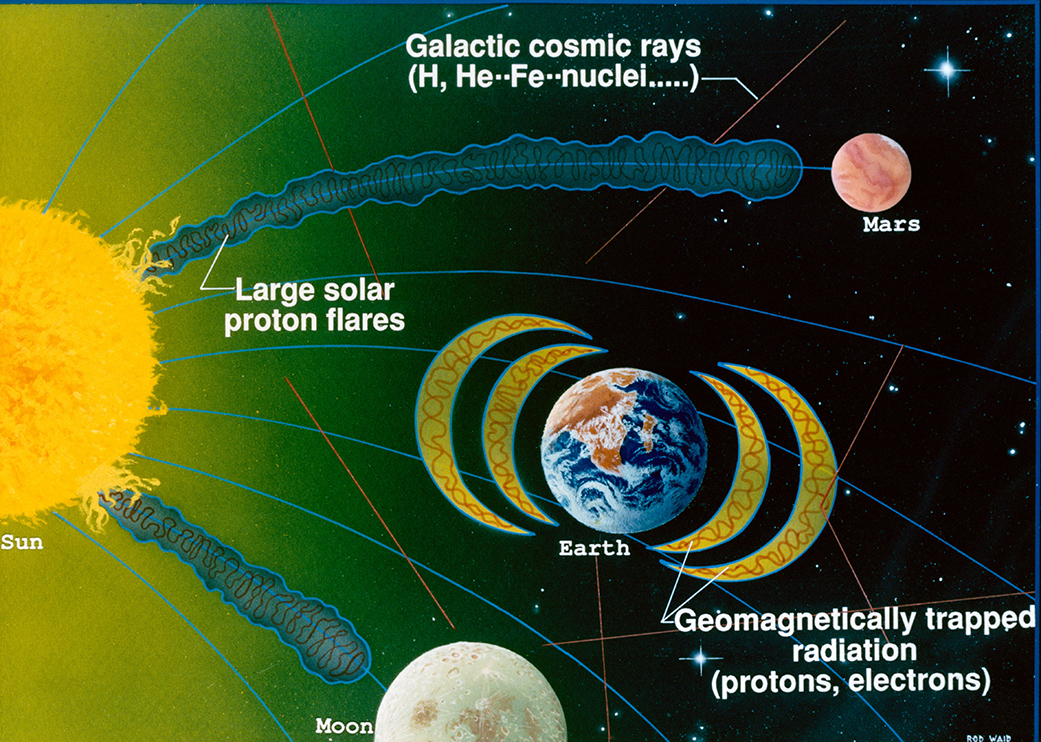
\includegraphics[scale=0.80]{figures/fig4_5.jpg}
			%\caption{}
		\end{figure}   
    \begin{itemize}
\item \textcolor{blue}{Solar Particle Events}:
\begin{itemize}
\item \textcolor{red}{Spettro}:
\begin{itemize}
\item 90$\%$ protoni
\item 10$\%$ ioni pesanti
\end{itemize}
\item  \textcolor{red}{Flusso}: $\approx$ $10^{10}$ part/($cm^{2}$ $s$ $sr$) al minimo solare
\item  \textcolor{red}{Dose} $\approx$ Sv/day \newline
 (fortemente dipendente dalla schermatura e dall'organo)
\end{itemize}
\end{itemize}

       %\begin{figure}
	%		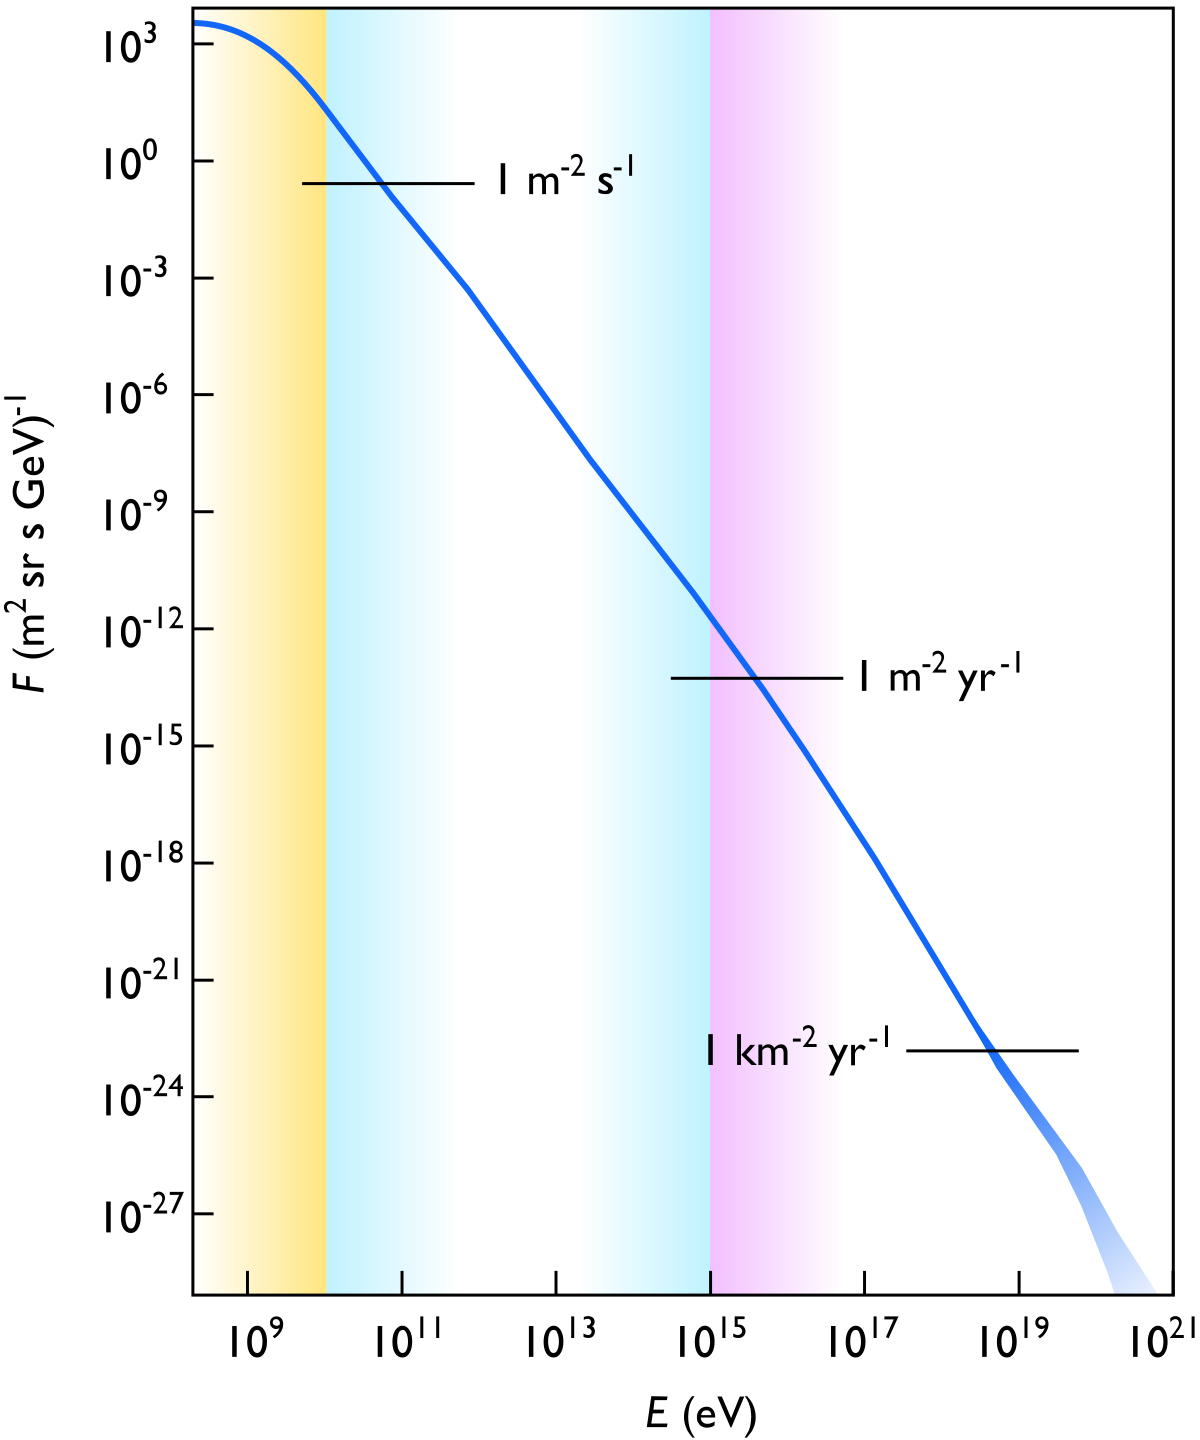
\includegraphics[scale=0.11]{figures/fig1_3.png}
	%		\caption{Rappresentazione della radiazione cosmica.}
	%	\end{figure}
    \end{column}
\end{columns}


\end{frame}

%==================================================================
				%SLIDE - Il campo di radiazione nello spazio - CGR
%==================================================================

\subsection{Radiazione cosmica galattica}
\begin{frame} [fragile]
\small
	\frametitle{Radiazione cosmica galattica - CGR}
\begin{columns}
  \begin{column}{0.50\textwidth}
\begin{figure}
	  \centering
			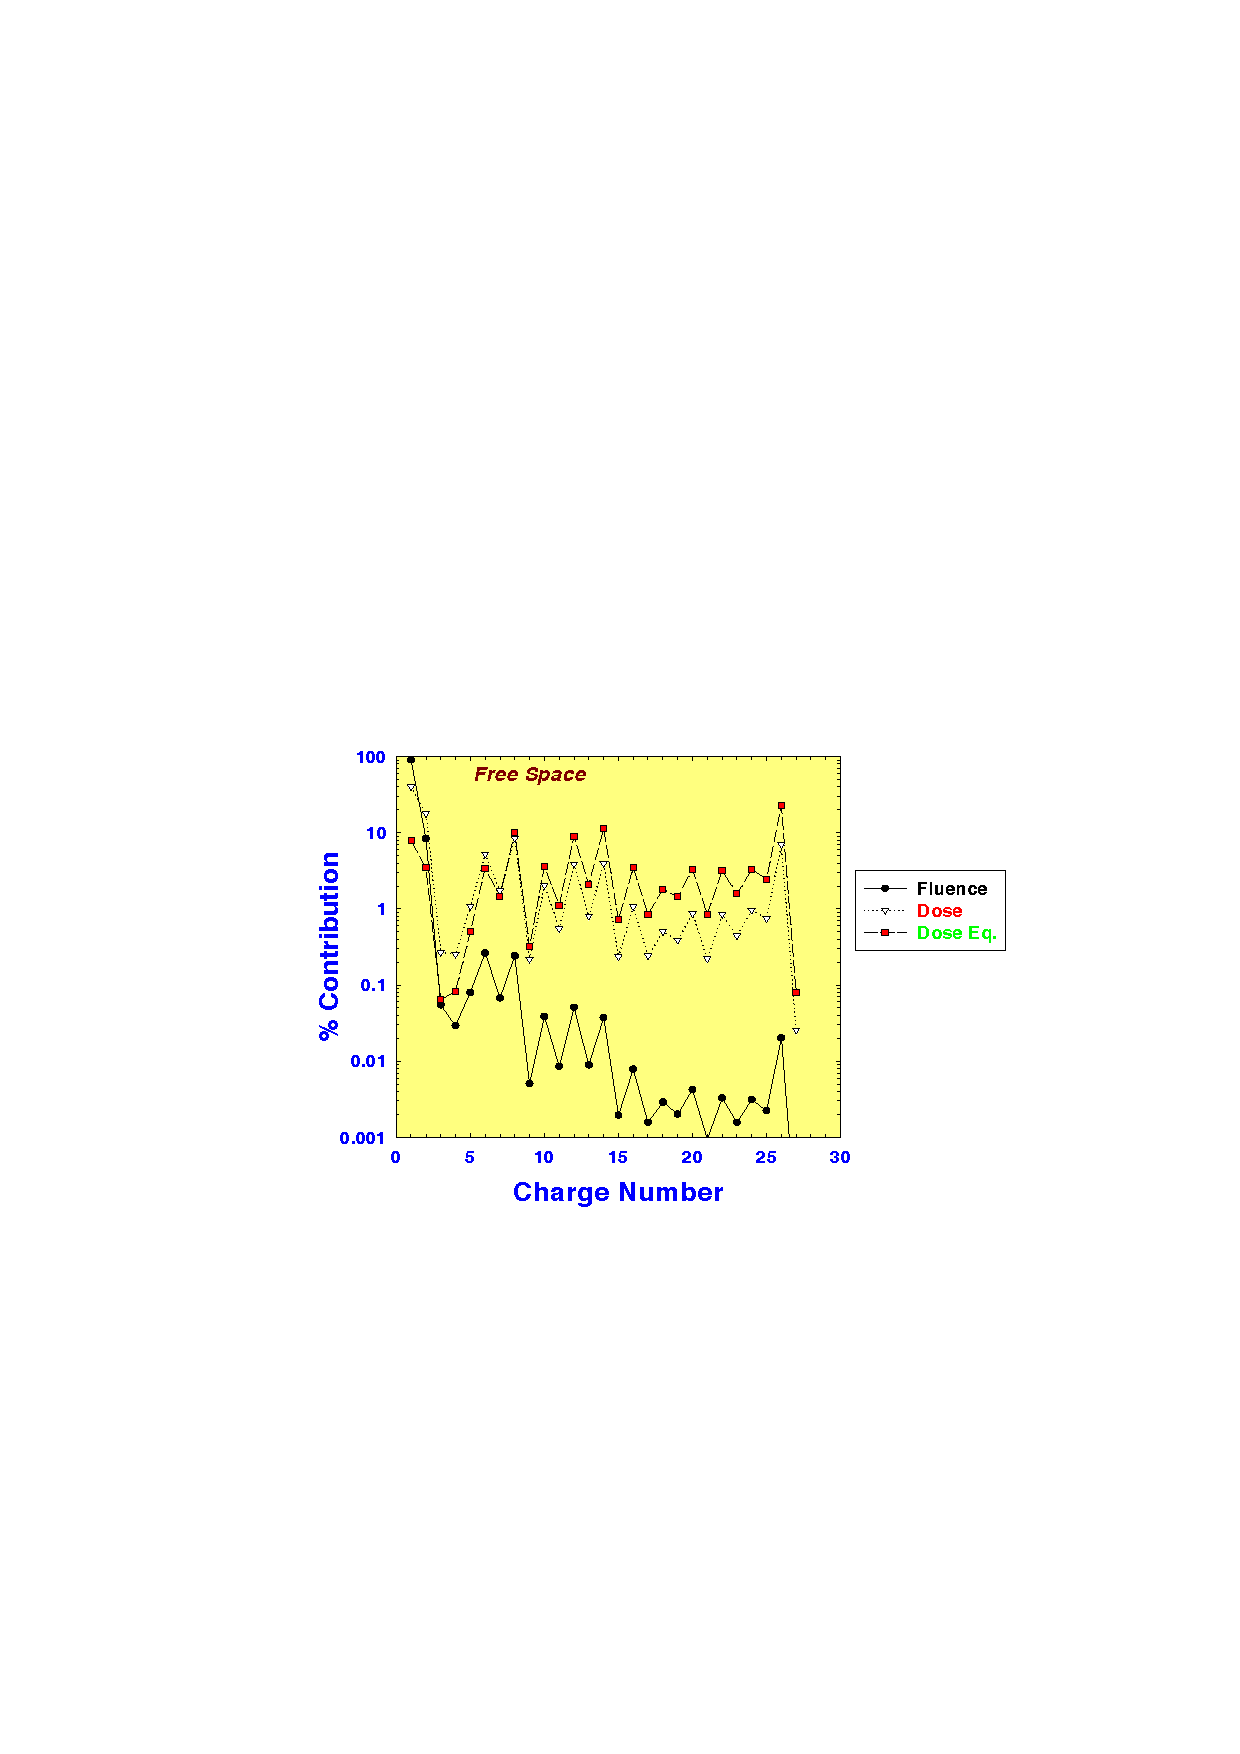
\includegraphics[scale=.55]{figures/fig2_2.pdf}
			\caption{Contributo dei CGR dalle differenti particelle}
		\end{figure}
	 \end{column}
    \begin{column}{0.50\textwidth}
 \newline
\begin{figure}
	  \centering
			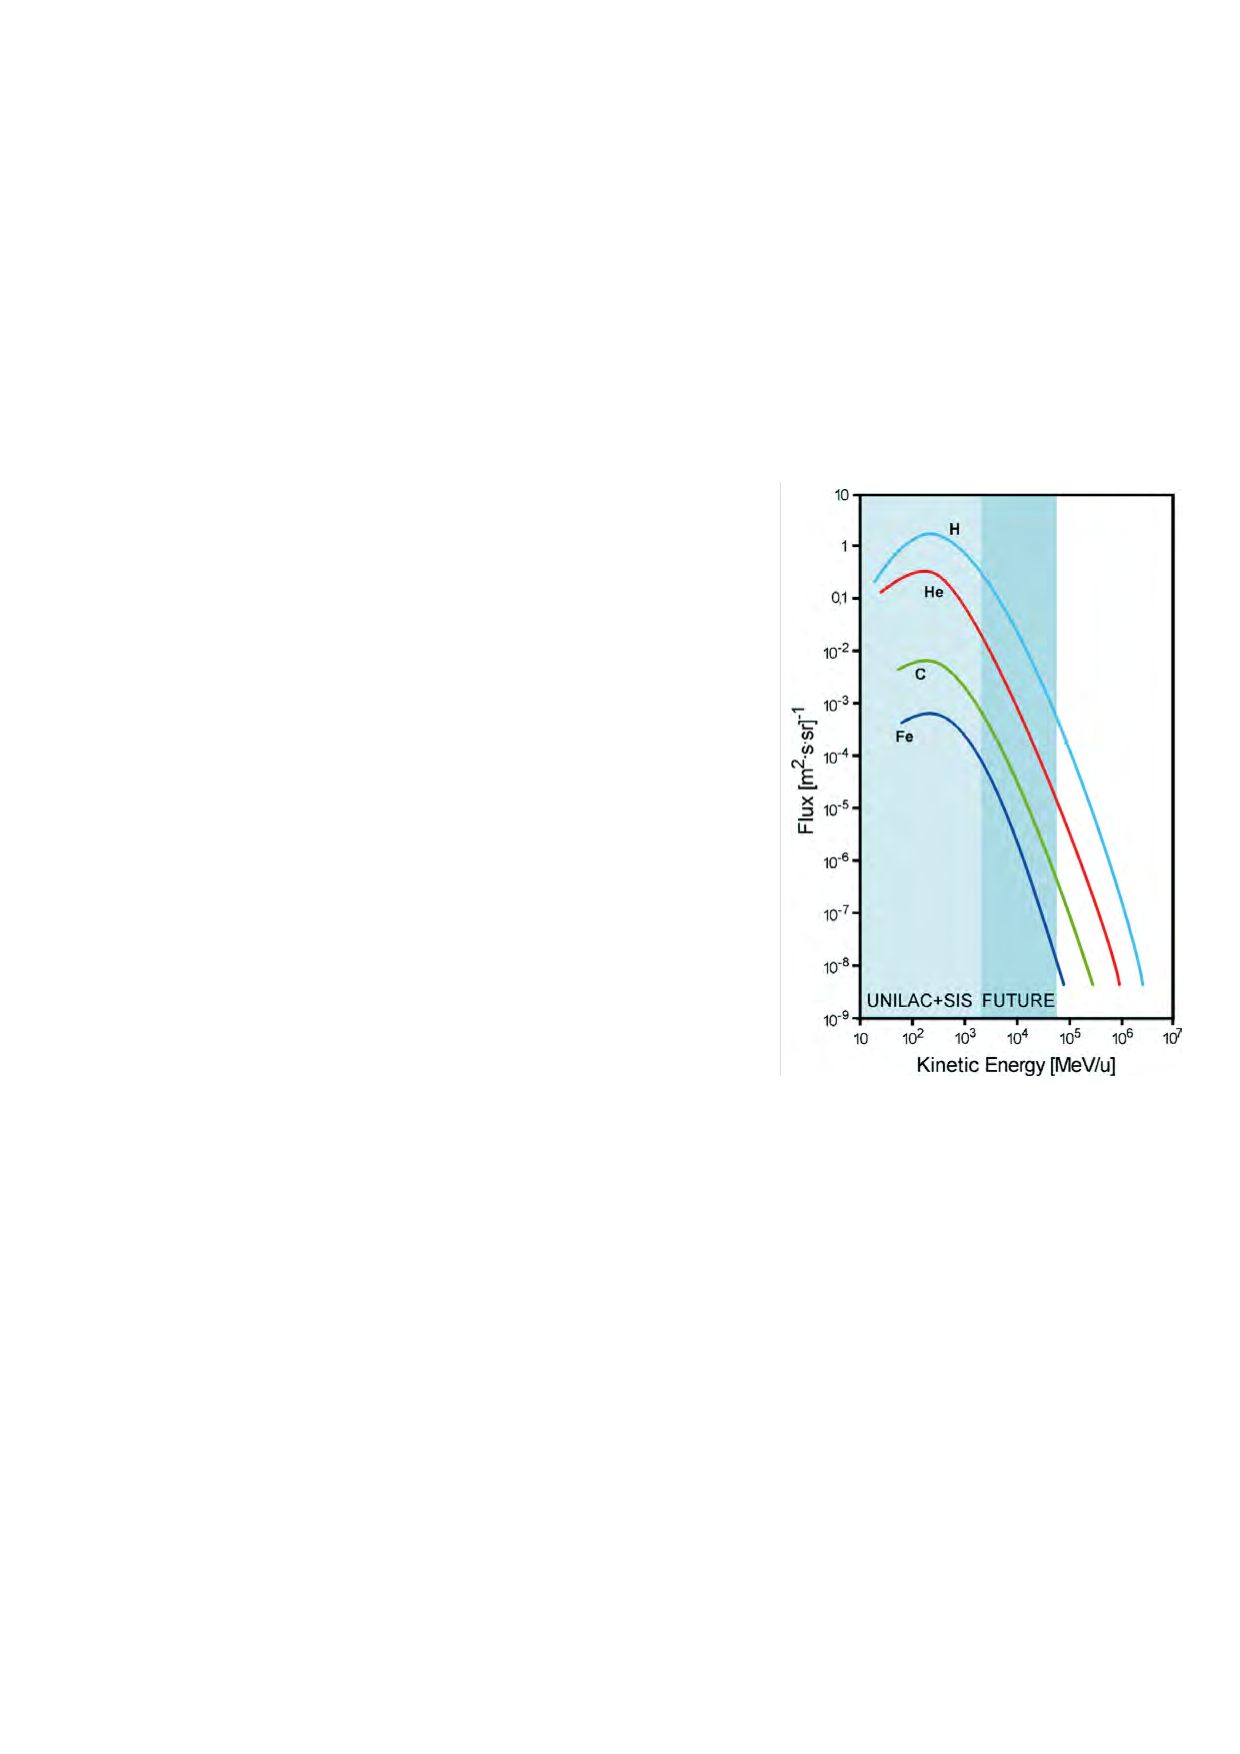
\includegraphics[scale=.55]{figures/sagg1.pdf}
			\caption{Spettri energetici di diversi ioni nei GCR \cite{saggiatore}}
		\end{figure}
    \end{column}
\end{columns}
\end{frame}
	
%==================================================================
					%SLIDE - Eruzioni solari - SPE
%==================================================================

\subsection{Eruzioni solari}
\begin{frame} [fragile]
		\frametitle{Eruzioni solari - SPE}
		
Il Sole emette una radiazione di natura particellare costituita dal \textcolor{blue}{vento solare}
Flusso di particele con velocit\`a di 300 $\div$ 800 km/s $\Longrightarrow$ $E$ $\approx$ 100 eV $\div$ 3.5 keV
\newline

Occasionali \textcolor{blue}{esplosioni superficiali} + \textcolor{blue}{intensi campi magnetici} della corona solare accelerano la materia $\Longrightarrow$ \colorbox{yellow}{Solar Particle Events}.

Intense esplosioni solari che iniettano alti flussi di particelle cariche, costituite per il 90$\%$ da protoni ed il restante 10$\%$ da $He$ ed ioni pesanti, nello spazio interplanetario con $E$ $\approx$ GeV 
\newline

\colorbox{pink}{Durata} poche $h$ $\div$ qualche settimana 
\newline

La \colorbox{pink}{pericolosit\`a degli SPE} dipende dal flusso $p$ di alta energia ($>$100 MeV) \textcolor{blue}{difficilmente schermabili} (e da prevedere!) 
\newline
Maggior contributo alla $D_{eq}$ prodotta da SPE $\sim$ 90$\%$
\end{frame}
	
%==================================================================
					%SLIDE - Radiazione Confinata TP
%==================================================================

\subsection{Radiazione Confinata $TP$}
\begin{frame} [fragile]
\small
	\frametitle{Radiazione Confinata $TP$}
\begin{figure}
	  \centering
			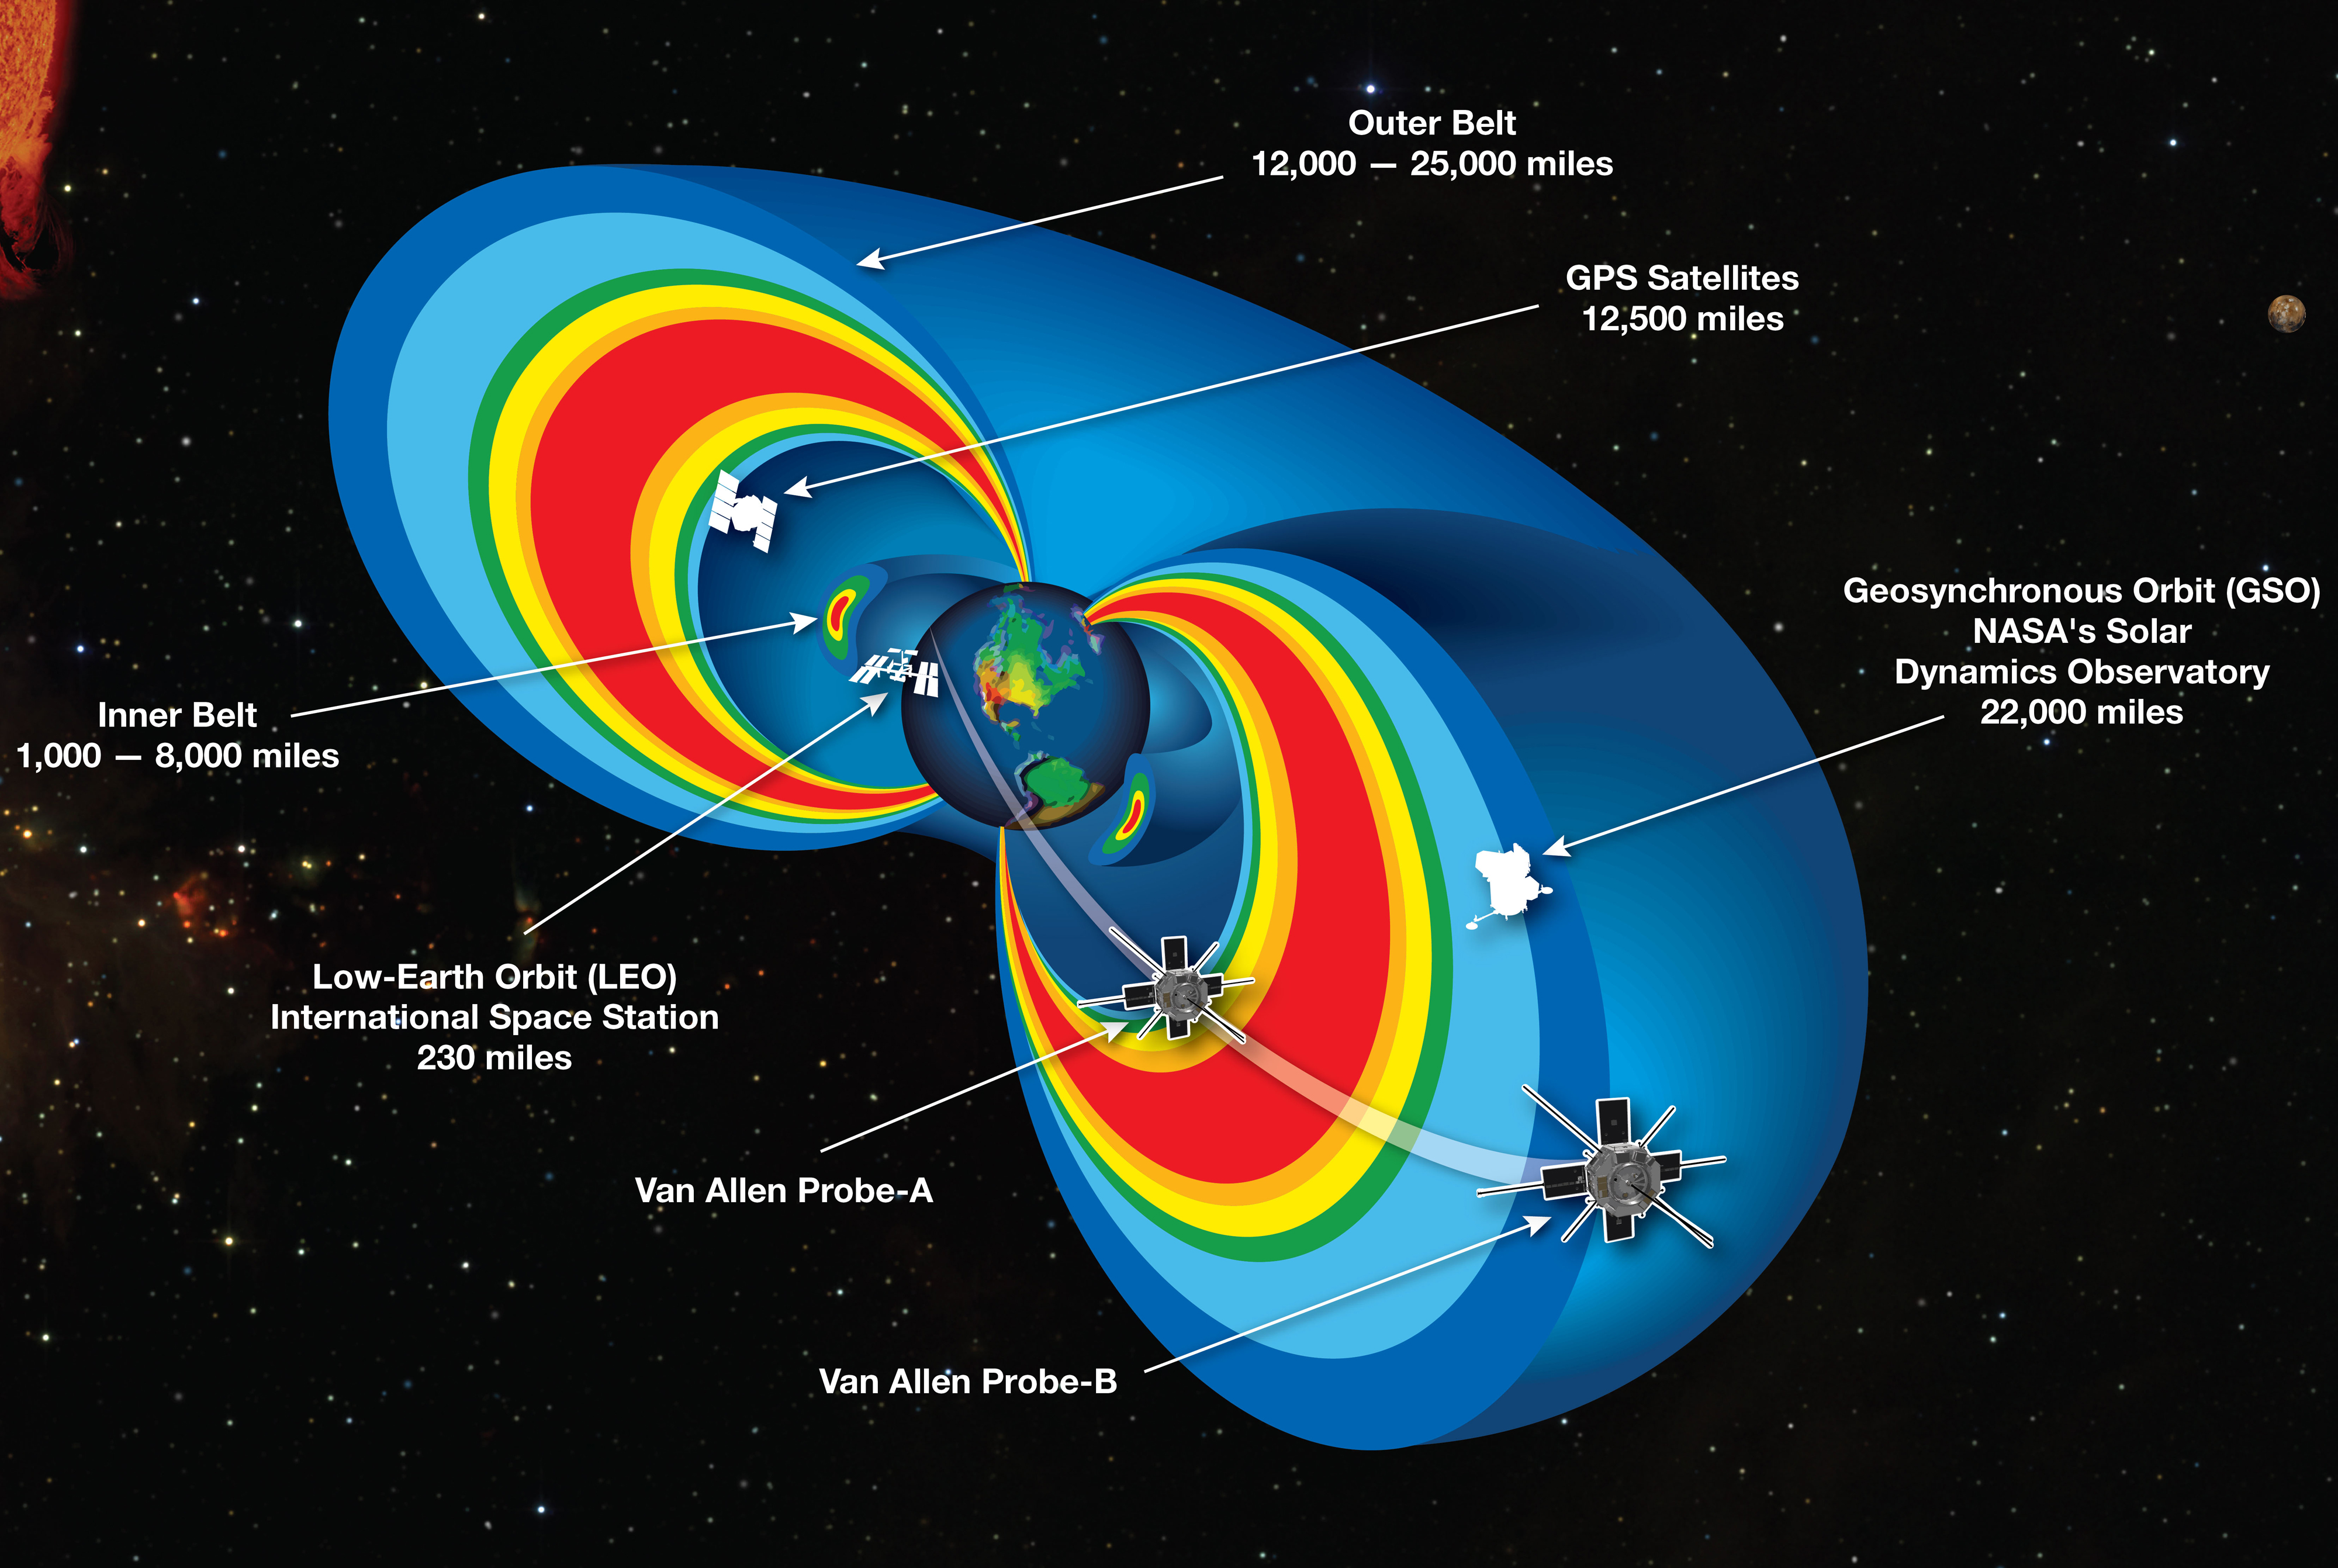
\includegraphics[scale=0.20]{figures/fig1_2.jpg}
			\caption{Trapped radiation:  Van Allen belts}
		\end{figure}
%Le cinture di radiazione sono due regioni a forma di ciambella che circondano la Terra, dove particelle ad alta energia, principalmente $e^{-}$ e ioni, sono intrappolate dal campo magnetico terrestre.
%Influisce sulle prestazioni delle  tecnologie e costituisce una minaccia per gli astronauti e i veicoli spaziali.
Le particelle che la compongono, prevalentemente \textcolor{blue}{protoni} ed \textcolor{blue}{elettroni energetici} (da 40 keV a 600 MeV), ma anche alcuni \textcolor{blue}{ioni pi\`u pesanti}, sono raccolte in regioni concentriche a forma d'anello che si estendono sopra l'atmosfera ($h$ = 1.6 $\div$ 40.0 km)
\end{frame}
	
%==================================================================
			%SLIDE - Effetti biologici della radiazione nello spazio
%==================================================================

\section{Effetti biologici della radiazione nello spazio}
{\usebackgroundtemplate 
{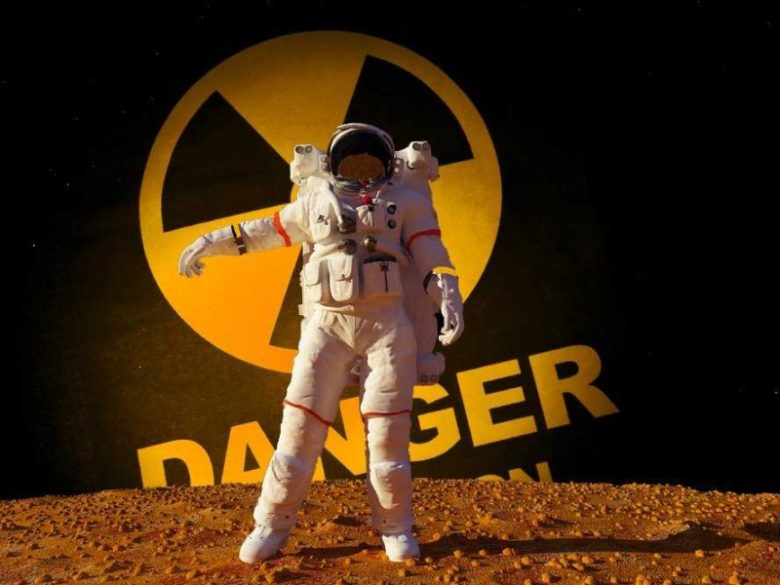
\includegraphics[width=\paperwidth]{figures/fig0.jpg}}
\begin{frame} [fragile]
	\frametitle{Effetti biologici della radiazione nello spazio}

\end{frame}
}
	
%==================================================================
				%SLIDE - Rischi da radiazione nello spazio
%==================================================================

\subsection{Rischi da radiazione nello spazio}
\begin{frame} [fragile]
	\frametitle{Rischi da radiazione nello spazio}
Per valutare la pericolosit\`a dell'esposizione alla radiazione \`e necessario considerare due grandezze:
\begin{itemize}
\item \textcolor{red}{Dose assorbita}, ossia la quantit\`a di energia depositata dalle radiazioni per unit\`a di massa \footnote{Negli USA la dose assorbita viene misurata in $[rad]$ (Radiation Absorbed Dose), mentre nel S.I. viene misurata in $[Gy]$} $D$ $=$ $d\varepsilon$$/$$dm$ 
\item \textcolor{red}{Dose equivalente}, che tiene conto del danno biologico che i differenti tipi di radiazione sono in grado di infliggere\footnote{Misurata in $[Sv]$} $H_{T}$ $=$ $\sum_{R}^{}$ $w_{R}$ $D_{T,R}$ 
\end{itemize}

%I rischi per la salute associati all'esposizione alle radiazioni spaziali sono stati discussi in numerosi rapporti e pubblicazioni e possono essere essenzialmente divisi in quattro gruppi:
\begin{block}{Rischi per la salute associati all'esposizione alle radiazioni spaziali \cite{saggiatore}}
\begin{itemize}
\item Cancro
\item Effetti tardivi (stocastici) degenerativi dei tessuti
\item Sindromi da radiazioni acute (i sistemi ematopoietico, gastrointestinale, cutaneo e neurovascolare).
\item Effetti ereditari
\end{itemize}
\end{block}
\end{frame}
	
%==================================================================
				%SLIDE - Rischi da radiazione nello spazio
%==================================================================

\begin{frame} [fragile]
	\frametitle{Rischi da radiazione nello spazio}
	\begin{exampleblock}{NASA Education - Space faring: The radiation challenge - Mod. 1, p. 8}
\begin{center} 
\scalebox{0.80}{ 
\begin{tabular}{lcc}
\hline
\hline
 \textbf{Mission type} &  \textbf{Radiation Dose} $[mSv]$   \\
\hline
\hline
       Space Shuttle 41C (8-day orbiting the Earth at 460 km)	        &   5.59       \\
       Skylab (87-day orbiting the Earth at 473 km)       			&   11.4       \\
       Skylab 4 (87-day orbiting the Earth at 473 km)      			&   178        \\
       ISS (up to 6 orbiting Earth at 353 km)                       			&   160        \\
       Estimated Mars            								&   1200     \\
\hline
\hline
\end{tabular}
 }
\linebreak
\end{center} 
\end{exampleblock}
	\begin{alertblock}{Missione Skylab 4}
	In soli tre mesi gli occupanti della stazione spaziale hanno accumulato una dose di radiazioni simile a quella che, per effetto del fondo naturale, un italiano\footnote{Mediamente noi italiani siamo annualmente esposti a 3.3 mSv. La media mondiale \`e di 2.4 mSv annui} accumulerebbe in quasi 54 anni.
\end{alertblock}

%\`E evidente come l'aumento dei tempi di esposizione renda ancora pi\`u critica la situazione.
%\newline

\url{https://www.scienzainrete.it/articolo/spazio-radiazioni-pi%C3%B9-pericolose-del-previsto/claudio-elidoro/2017-07-26}
\end{frame}

%==================================================================
			%SLIDE - Rischi da radiazione nello spazio
%==================================================================

\begin{frame} [fragile]
	\frametitle{Rischi da radiazione nello spazio}
	\small
\begin{block}

\begin{itemize}
\item Dose eq. \textcolor{blue}{Terra} = 10 $\mu$Sv/d
\item Dose eq. \textcolor{orange}{Luna} = 100 $\div$ 200  $\mu$Sv/d

\item Dose eq. \textcolor{red}{Missione per Marte} (9 mesi) = 1.2 Sv \newline
$\Longrightarrow$ \textcolor{blue}{\textit{What Happens to Your Brain on the Way to Mars}} \url{https://www.researchgate.net/publication/275866556}
\end{itemize}
\end{block}

\begin{itemize}
\item  \colorbox{pink}{1 $\div$ 2 Sv} \colorbox{yellow}{Avvelenamento radioattivo lieve} $\Longrightarrow$ 10$\%$ di mortalit\`a dopo 30 d\'i
\item \textcolor{red}{Sintomi tipici} includono \textcolor{blue}{nausea} da lieve a moderata (con un 50$\%$ di probabiliit\`a a 2 Sv), con vomito occasionale, che comincia da 3 a 6 ore dopo l'irraggiamento e permane per circa un giorno. 
\item Seguito da una \textcolor{blue}{fase latente} che dura \textcolor{blue}{da 10 a 14 giorni}, quando appaiono \textcolor{blue}{sintomi lievi di astenia e malessere generale} (con un 50$\%$ di probabilit\`a ai 2 Sv).
\item Il sistema immunitario va incontro a depressione $\Longrightarrow$ \textcolor{blue}{periodo di convalescenza} esteso per molte \textcolor{blue}{infezioni} comuni e un aumento del rischio di infezione opportunistica.
\item Uomo: comune la \textcolor{blue}{sterilit\`a temporanea}. 
\item Donna: \textcolor{blue}{Aborto spontaneo} oppure aumento di incidenza del parto prematuro si verifica comunemente nelle donne incinte.

\end{itemize}
\end{frame}

	
%==================================================================
				%SLIDE -  Effetti sugli astronauti
%==================================================================
%\begin{frame} [fragile]
%	\frametitle{Effetti sugli astronauti}
%		\begin{figure}
%	  		\centering
%				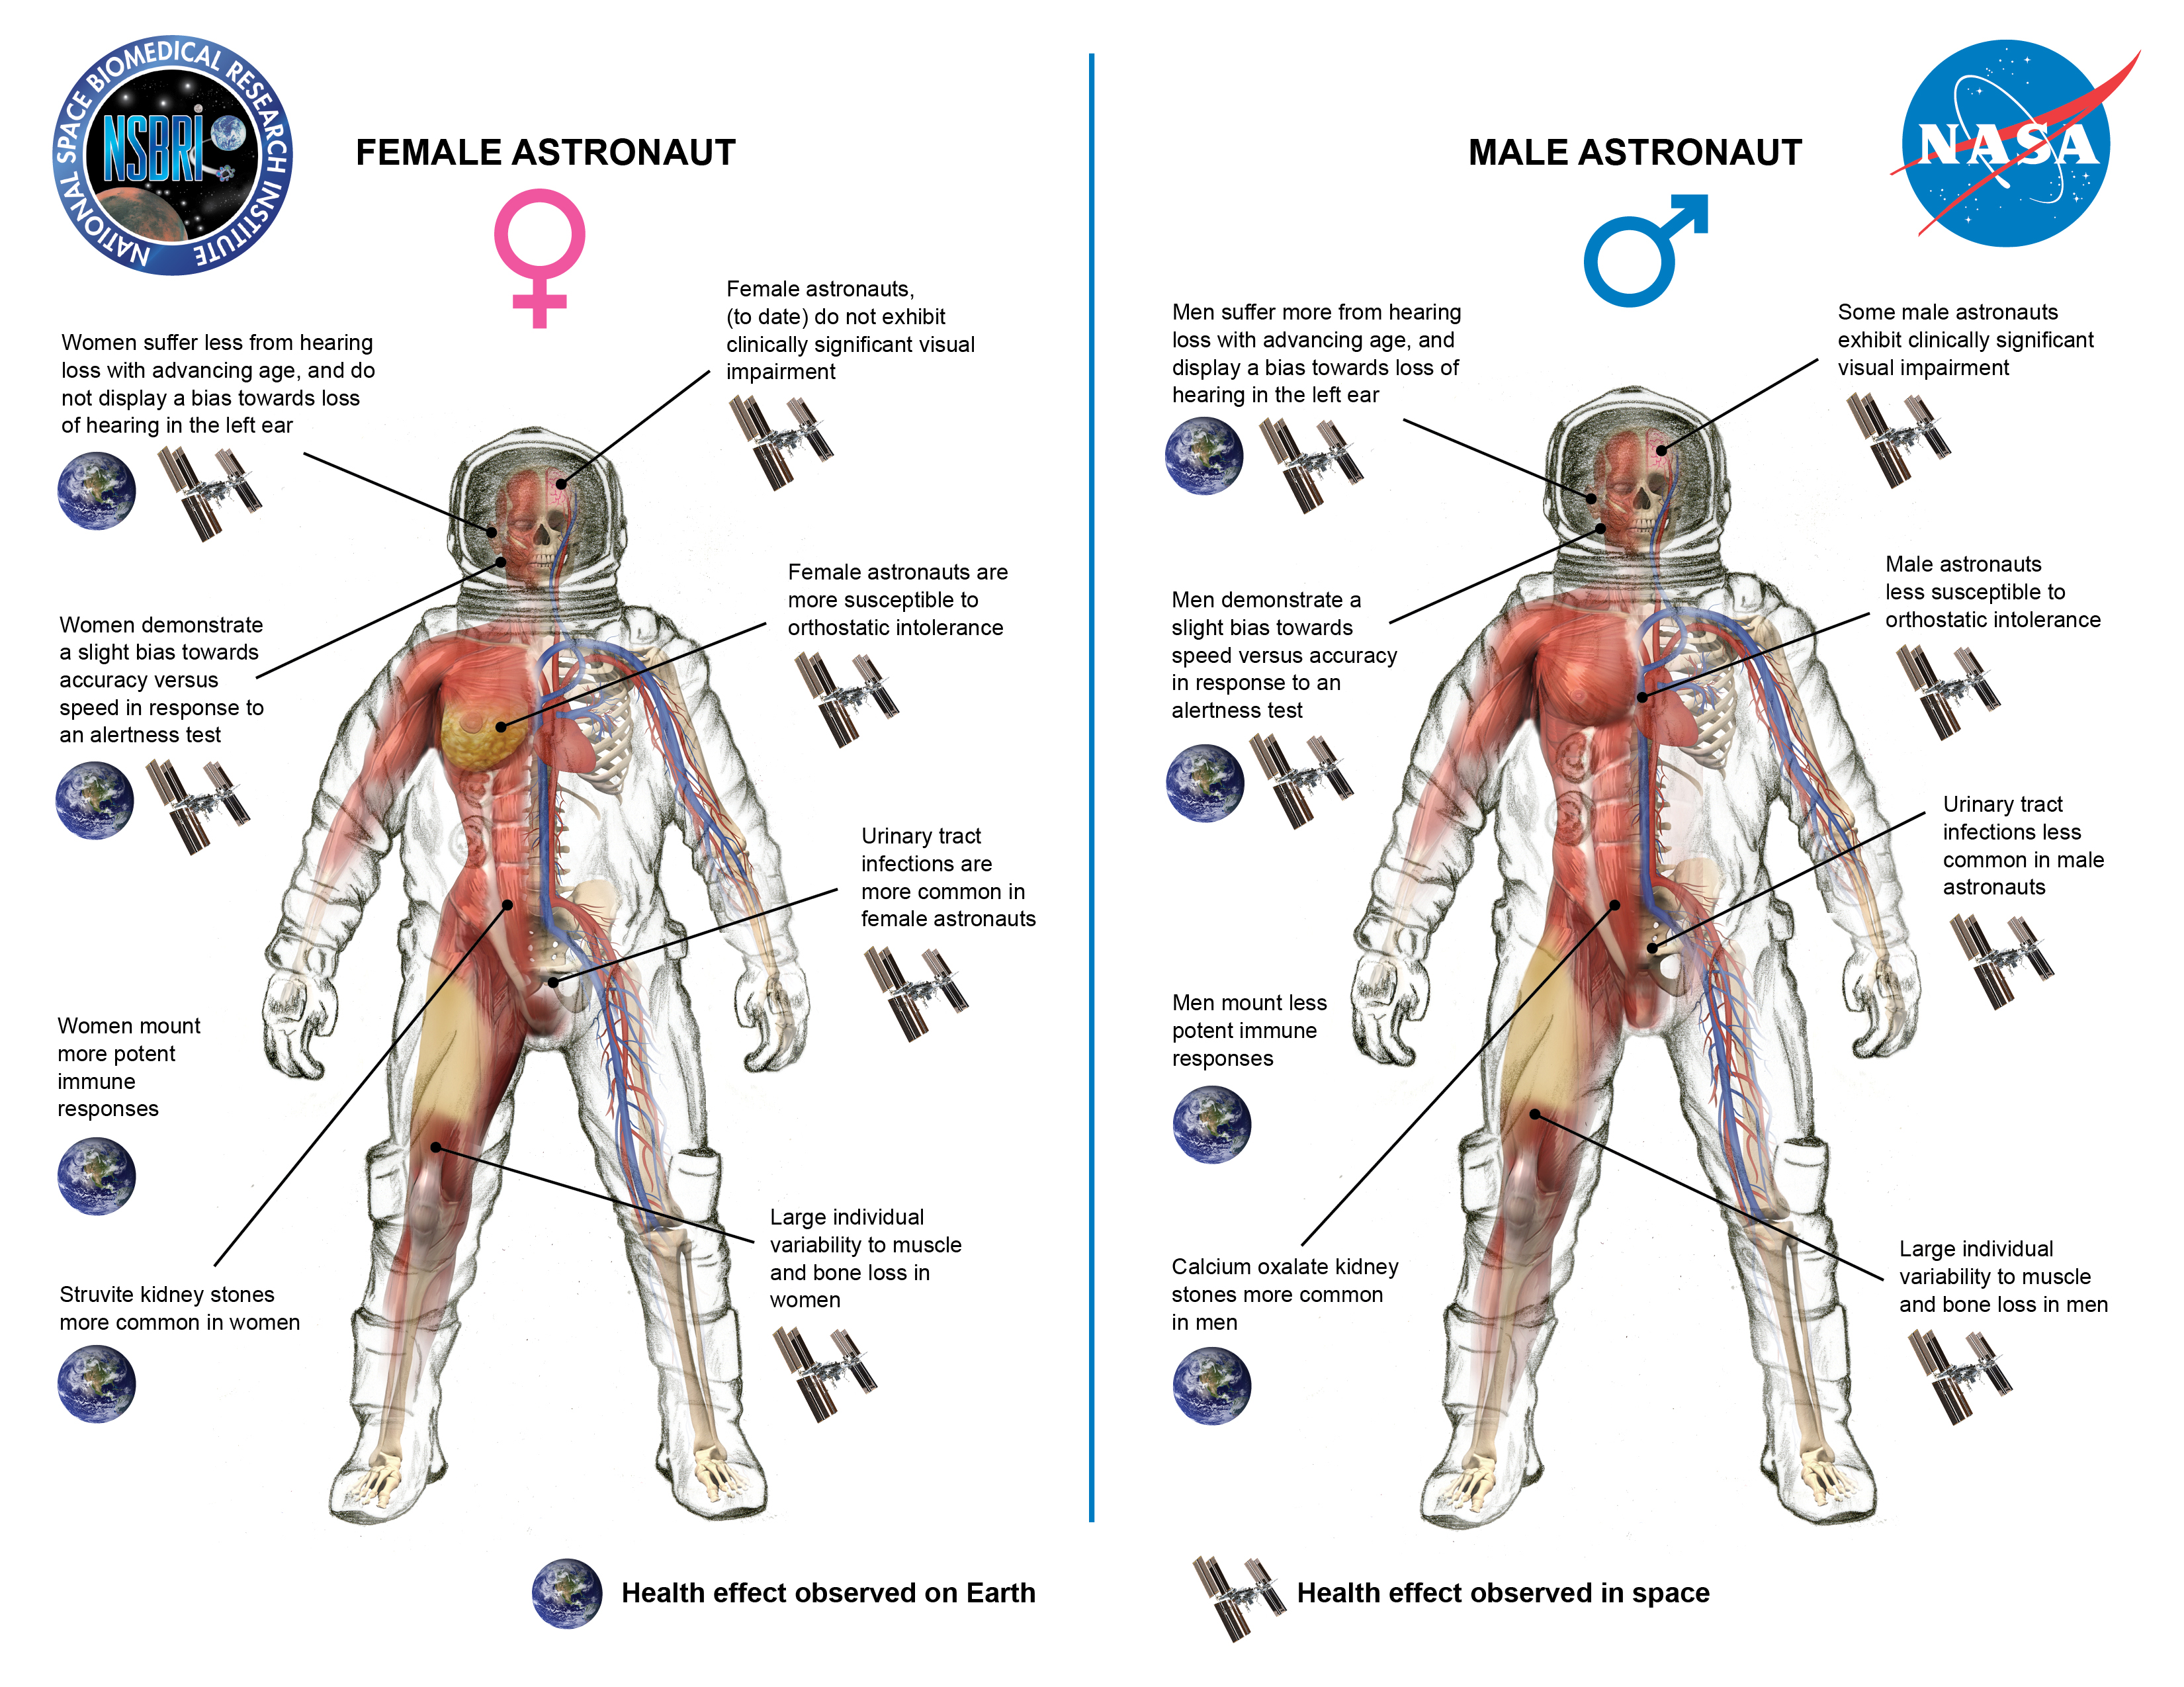
\includegraphics[scale=0.36]{figures/fig3_3.jpeg}
%				%\caption{Trapped radiation:  Van Allen belts}
%		\end{figure}
%\end{frame}
	

	


%==================================================================
				%SLIDE - Rischi da radiazione nello spazio
%==================================================================

\begin{frame} [fragile]
	\frametitle{Rischi da radiazione nello spazio}
\begin{block}{}
\centering
Effetti ed eventuali \textcolor{red}{danni recati a tutte le apparecchiature di bordo}
\end{block}

Effetti sono catalogabili in \textcolor{blue}{effetti irreparabili} e \textcolor{blue}{temporanei:} i primi si riscontrano soprattutto nelle apparecchiature dotate di transistors (semiconduttori), i secondi, invece, influenzano le memorie e i registri inducendo dei \textcolor{blue}{cambiamenti nei bits} ($spin-flip$ delle memorie logiche) e quindi  \textcolor{blue}{cambiamenti nelle informazioni registrate}.
\newline

Tali effetti possono limitare enormemente la durata di una missione spaziale.
\newline

%Altre conseguenze meno catastrofiche, ma non per questo trascurabili, sono la  \textcolor{blue}{creazione di interferenze nei dispositivi elettronici} $\Longrightarrow$ degrado dell'efficienza della missione. 
\end{frame}


\begin{frame} [fragile]
\begin{figure}
	  \centering
			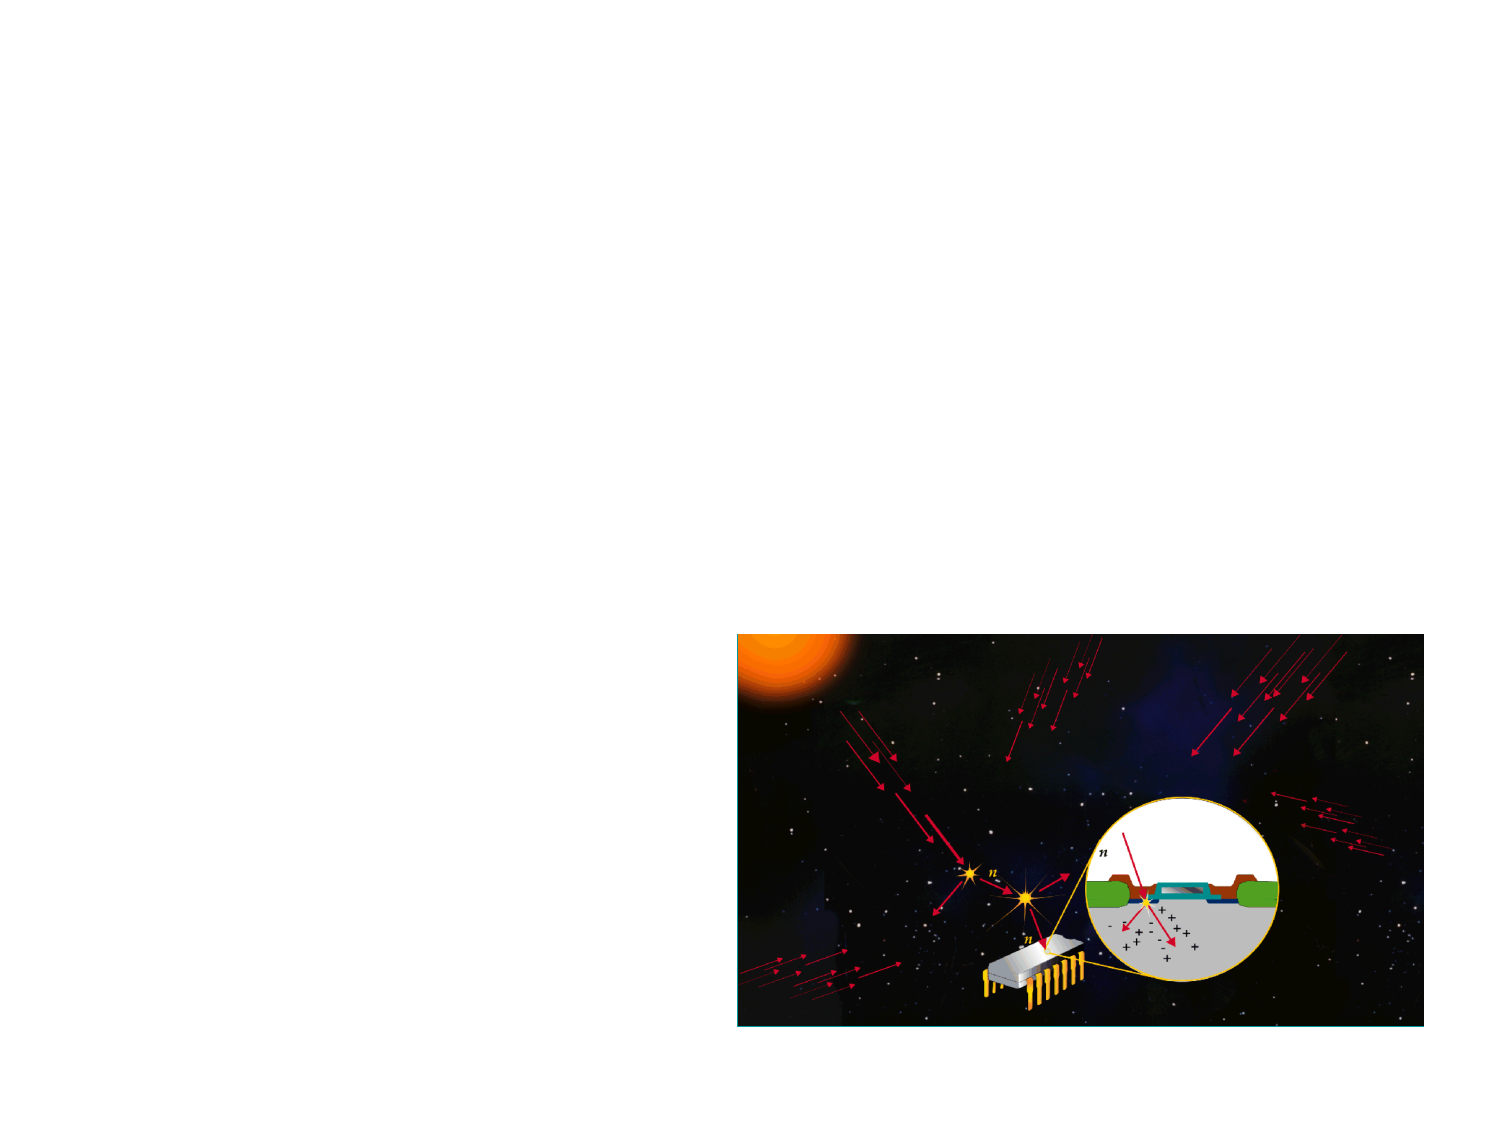
\includegraphics[scale=0.80]{figures/fig3_3.pdf}
			%\caption{Radiation Belts $h$ = 1.6 $\div$ 40.0 km }
		\end{figure}

Altre conseguenze meno catastrofiche, ma non per questo trascurabili, sono la  \textcolor{blue}{creazione di interferenze nei dispositivi elettronici} $\Longrightarrow$ degrado dell'efficienza della missione. 

\end{frame}


%==================================================================
						%SLIDE - Calcoli di dose
%==================================================================

\begin{frame} [fragile]
	\frametitle{Calcoli di dose}
		\begin{figure}
	  \centering
			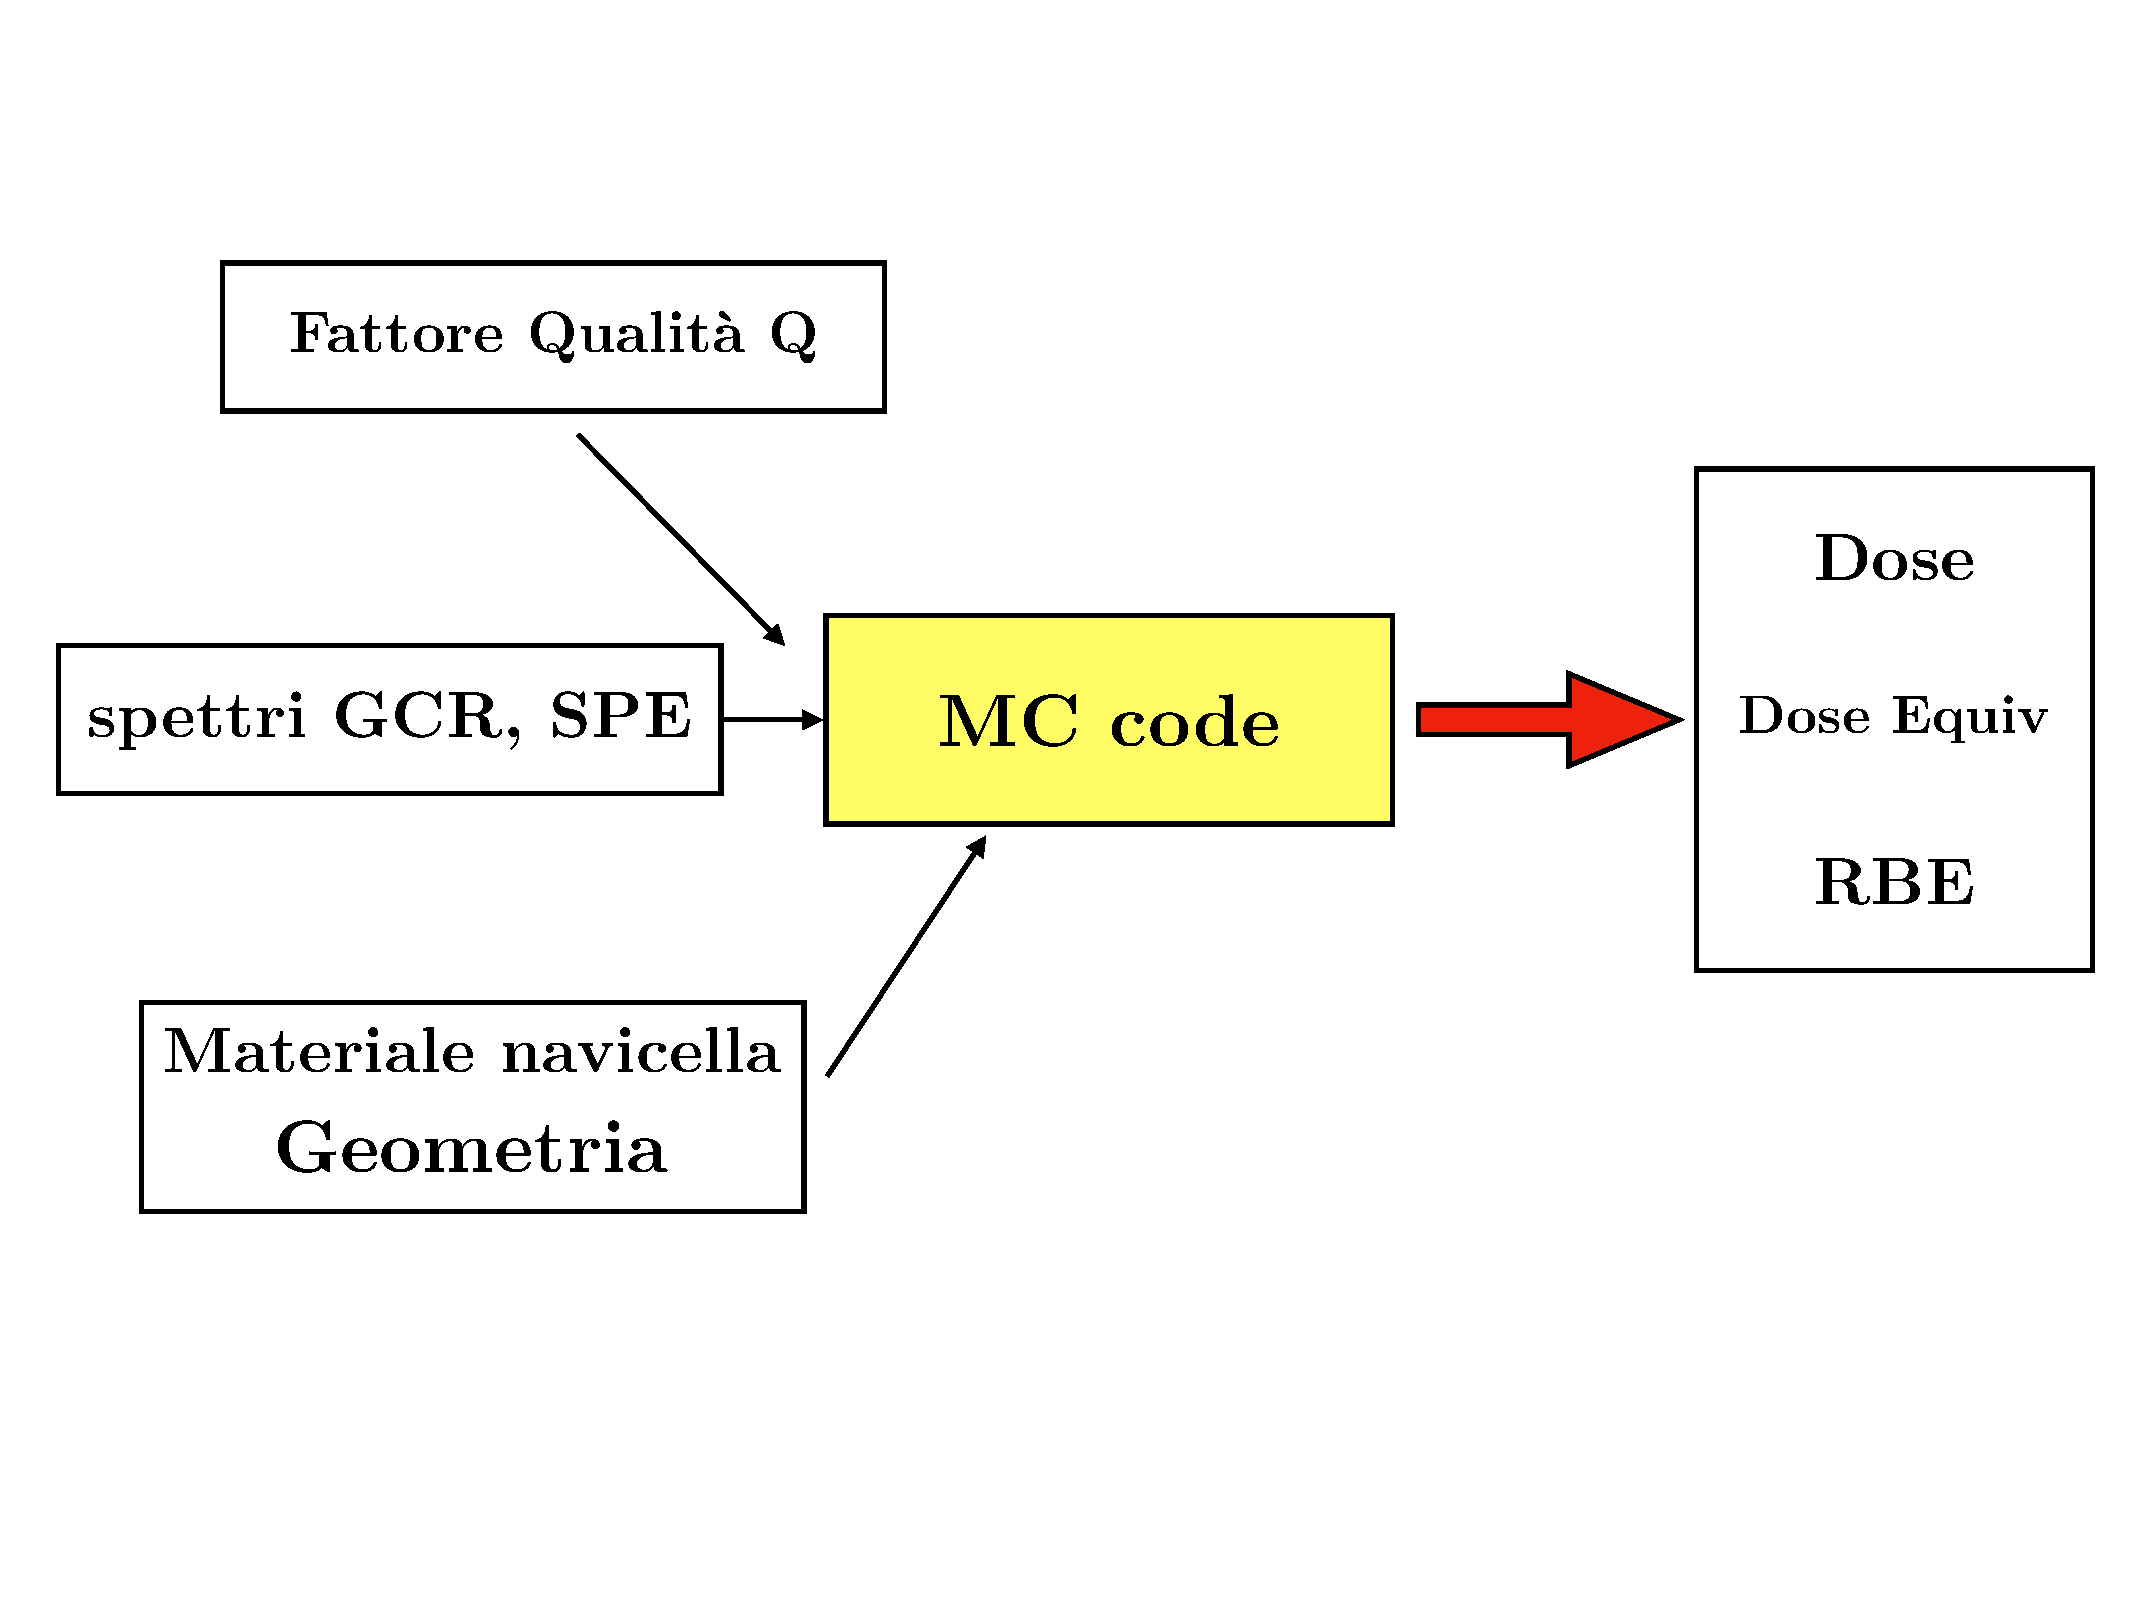
\includegraphics[scale=0.20]{figures/mc.pdf}
			%\caption{$\varphi$ angolo azimutale, $\vartheta$ angolo polare}
		\end{figure}

\begin{exampleblock}{Software principali}
\begin{itemize}
\item \texttt{FLUKA}
\item \texttt{GEANT4}
\item The High Energy Transport Code (\texttt{HETC}\footnote{\url{https://www.researchgate.net/publication/24383391_Verification_and_Validation_High_Charge_and_Energy_HZE_Transport_Codes_and_Future_Development}})
\end{itemize}
\end{exampleblock}

\end{frame}

%==================================================================
					%SLIDE - Protocolli di sicurezza
%==================================================================

\subsection{Protocolli di sicurezza}
\begin{frame} [fragile]
	\frametitle{Protocolli di sicurezza}
 A partire dagli anni '80 la NASA ha steso un piano normativo in linea con le regole dettate dall'OSHA\footnote{Occupational Safety and Health Administration, l'ente deputato alla sicurezza sul lavoro.}.
 \newline
 
 I protocolli NASA fissano un \textcolor{red}{limite massimo per l'esposizione a radiazioni ionizzanti} relativo all'intera carriera di un astronauta e stabiliscono che la \colorbox{yellow}{probabilit\`a di contrarre un cancro mortale a seguito di tale esposizione} debba essere \textcolor{blue}{inferiore al 3 $\%$} 
$\Longrightarrow$ tecnicamente si parla di \textcolor{red}{REID}\footnote{$Rrisk$ $Exposure$ $Induced$ $Death$}.	
\newline
%\pause
Molto complicato tradurre questo limite in quantit\`a di radiazione equivalenti valide in assoluto. Nella valutazione intervengono molti fattori:
\begin{itemize}
\item sesso
\item et\`a
\item sensibilit\`a dell'organismo alle radiazioni 
\item stile di vita dell'astronauta.
\end{itemize} 

  \end{frame}
  
%==================================================================
					%SLIDE - Protocolli di sicurezza
%==================================================================

\begin{frame} [fragile]
	\frametitle{Protocolli di sicurezza}
	Nella seguente tabella\cite{Nasa1} possiamo leggere i \textcolor{red}{limiti massimi di radiazione per l'intera carriera} stabiliti dalla NASA a seconda dell'et\`a degli astronauti e del loro genere:
 \begin{exampleblock}{Career Exposure Limits for NASA Astronauts by Age and Generd}
\begin{center}
\scalebox{0.90}{ 
\begin{tabular}{lccccc}
\hline
\hline
 \textbf{Age(years)} & 25  &   35 &   45 &   55   \\
\hline
\hline
       Male        	&   1500 mSv      &   2500 mSv  &   3250 mSv &   4000 mSv   \\
       Famale      &   1000 mSv      &   1700 mSv  &   2500 mSv &   3000 mSv   \\
\hline
\hline
\end{tabular}
 }
\linebreak
\end{center} 
\end{exampleblock}

%\colorbox{cyan}{\textcolor{withe}{OSS:}}
%\colorbox{yellow}{OSS:}
%\newline
I valori sono pi\`u bassi per gli astronauti pi\`u giovani. 
\newline

Si presume che, sebbene possano vivere pi\`u a lungo degli astronauti pi\`u anziani, l'esposizione a maggiori quantit\`a di radiazioni nelle prime fasi della loro carriera potrebbe presentare maggiori rischi per la salute durante la vecchiaia.

\end{frame}
	
%==================================================================
					%SLIDE - Protocolli di sicurezza
%==================================================================

\begin{frame} [fragile]
	\frametitle{Protocolli di sicurezza }
 \begin{exampleblock}{Depth of Radiation Penetration and Exposure Limits for Astronauts and the General Public [$mSv$]}
\begin{center}
\scalebox{0.60}{ 
\begin{tabular}{lccccc}
\hline
\hline
 			 & Exposure Interval  &   Blood Forming Organs (5 cm depth) &   Eyes (0.3 cm depth) &   Skin (0.01 cm depth)   \\
\hline
\hline
               			&   30 Days     &   250  		 &   1000 &   1500   \\
       Famale     		&   Annual       &   500		 &   2000 &   3000   \\
       				&   Career       &   1000-4000    	&   4000 &   6000   \\
\hline
  General Public     	&   Annual       &   1			 &   15 &   50   \\
\hline
\hline
\end{tabular}
 }
\linebreak
\end{center} 
\end{exampleblock}
%\textcolor{blue}{Integrative Risks Models Toolkit}
\begin{alertblock}{Integrative Risks Models Toolkit}
\begin{itemize}
\item \texttt{ARRBOD} $\Longrightarrow$ Acute Radiation Risk and BRYNTRN Organ Dose
\item \texttt{GERMCode} $\Longrightarrow$ GCR Event-based Risk Model
\item \texttt{NASARTI}   $\Longrightarrow$ NASA Radiation Track Image
\item ...
\end{itemize}
\end{alertblock}
\url{https://www.nasa.gov/hrp/elements/radiation/irModels}

\end{frame}
	
%==================================================================
					%SLIDE - Protocolli di sicurezza
%==================================================================

\begin{frame} [fragile]
	\frametitle{Protocolli di sicurezza}
	\begin{block}{}
	\center
Come si passa dalla \textcolor{red}{Dose} al \textcolor{red}{Rischio}  $\Longrightarrow$ \framebox{NASA radiation risk model}
\end{block}
%\newline

\small
Per una popolazione omogenea che riceve una dose efficace $E$, all'et\`a $a_{E}$, la \textcolor{red}{probabilit\'a di morire} nell'intervallo di et\`a da [$a$, $a$+1] \`e descritta dal \textcolor{blue}{tasso di mortalit\`a di fondo per tutte le cause di morte}, $M(a)$ e il \textcolor{blue}{tasso di mortalit\`a per tumore da radiazione} $m(E,a_{E}, a)$ come

\begin{equation*}
q(E, a_{E}, a) = \frac{M(a) + m(E, a_{E}, a)}{1 + \frac{1}{2}[M(a) + m(E, a_{E}, a)]}
\end{equation*}
\newline

La \textcolor{blue}{probabilit\`a di sopravvivenza} per vivere fino all'et\`a $a$, a seguito di esposizione $E$, all'et\`a $a_{E}$, sar\`a

\begin{equation*}
S(E, a_{E}, a) = \prod\limits_{u=a_{E}}^{a-1} [1-q(E,a_{E},u)]
\end{equation*}

\end{frame}
	
%==================================================================
					%SLIDE - Protocolli di sicurezza
%==================================================================

\begin{frame} [fragile]
	\frametitle{Protocolli di sicurezza}
	\begin{block}{}
	\center
Come si passa dalla \textcolor{red}{Dose} al \textcolor{red}{Rischio}  $\Longrightarrow$ \framebox{NASA radiation risk model}
\end{block}
%\newline

\small
Il \textcolor{red}{rischio di morte indotta da radiazione} (REID\footnote{Risk of Exposure Induced Death}) \`e il rischio per la vita che un individuo nella popolazione muoia per un cancro causato dalla sua esposizione alle radiazioni.

\begin{equation*}
\tcbhighmath[drop fuzzy shadow, ,watermark color=yellow!90!red]{
REID = \sum\limits_{a=a_{E}}^{a-1} m(E,a_{E},a) S(E,a_{E},a) }
\end{equation*}


dove
\begin{equation*}
m(E,a_{E},a) = [\nu ERR(a_{E},a) M_{c}(a) + (1 -\nu) EAR(a_{E}, a)] \frac{\sum\limits_{L} Q(L)F(L) L }{DDREF}
\end{equation*}

$ERR=E/C$ e $EAR=(E-C)$ in $Sv^{-1}$ derivano da sopravvissuti alla bomba atomica, $M$  \'e il tasso di mortalit\`a per cancro specifico per genere ed et\`a negli USA,\newline
 $\nu$ = 1/2 per il cancro solido e $\nu$ = 0 per la leucemia.

\end{frame}

	
%==================================================================
						%SLIDE - Detector
%==================================================================

\section{Detector}
\begin{frame} [fragile]
	\frametitle{Detector}
Una parte importante di ogni missione con equipaggio \`e la dosimetria delle radiazioni, ossia il \colorbox{yellow}{processo di monitoraggio}, \colorbox{yellow}{caratterizzazione} e \colorbox{yellow}{quantificazione della radiazione ambientale} in cui vivono e lavorano gli astronauti.
\newline 
   
Le missioni includono anche:
\begin{block}{}
\begin{itemize}
\item Stime calcolate dell'esposizione dell'equipaggio durante l'attivit\`a extra-veicolare
\item Valutazione di tutte le apparecchiature che producono radiazioni trasportate sul veicolo spaziale; 
\item Modellizzazione computerizzata completa dell'esposizione dell'equipaggio.
\end{itemize} 
\end{block}
%I membri dell'equipaggio della stazione spaziale indossano abitualmente dosimetri fisici per misurare la loro esposizione accumulata e, dopo il volo, forniscono un campione di sangue per misurare il danno da radiazioni ai cromosomi nelle cellule del sangue. 
\end{frame}


%==================================================================
				%SLIDE - RAD - Radiation Assessment Detector
%==================================================================
\subsection{RAD - $R$adiation $A$ssessment $D$etector}
\begin{frame} [fragile]
	\frametitle{RAD - $R$adiation $A$ssessment $D$etector}
\begin{columns}
  \begin{column}{0.50\textwidth}
\begin{figure}
	  \centering
			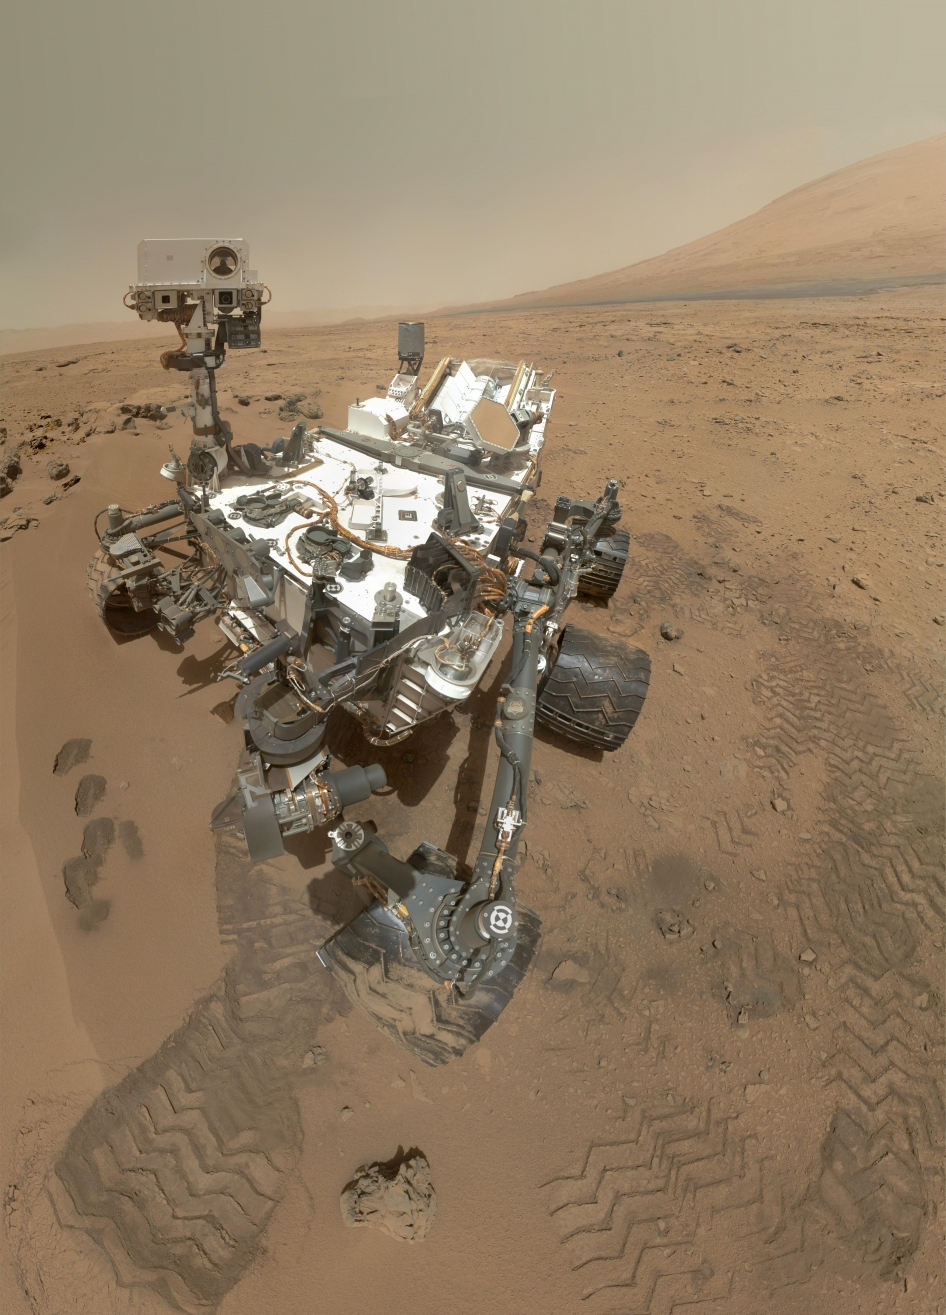
\includegraphics[scale=0.10]{figures/fig6_1.jpg}
			%\caption{ Rover Curiosity\newline
				 %Launch date: 26/11/2011\newline
				 %Landing date: 06/08/2012}
		\end{figure}
		\begin{block}{}
		\centering
		%Rover Curiosity\newline
		$\>$$\>$$\>$$\>$$\>$$\>$Launch date:$\>$$\>$ 26/11/2011\newline
		Landing date: 06/08/2012
		\end{block}
	 \end{column}
    \begin{column}{0.50\textwidth}
 Grande miglioramento proviene dalle misurazioni dello strumento \colorbox{pink}{Radiation Assessment Detector (RAD)}  trasportato dal \textcolor{red}{rover Curiosity} durante la missione su Marte. 
\newline

\colorbox{yellow}{La maggior parte della dose} \`e sostenuta \colorbox{yellow} {durante la fase di crociera}. 
\newline

La dose sul pianeta pu\`o essere ulteriormente ridotta usando basi con schermatura pesante, sfruttando materiali planetari in situ.
    \end{column}
\end{columns}
\end{frame}




%==================================================================
				%SLIDE - RAD - Radiation Assessment Detector
%==================================================================

\begin{frame} [fragile]
	\frametitle{RAD - $R$adiation $A$ssessment $D$etector}
\begin{columns}
  \begin{column}{0.50\textwidth}
Il 31 maggio 2013, gli scienziati della NASA hanno riportato i risultati ottenuti durante la crociera e hanno affermato che \colorbox{yellow}{il valore della dose equivalente} per il viaggio di sola andata e senza sosta ($t_{tot}$ $\sim$ $1$ anno) con i sistemi di propulsione e di schermatura attuali risulta essere  \colorbox{yellow}{0.66 $\pm$ 0.12 Sivert}. 
\newline

L'esposizione a 1 $Sv$ aumenta il rischio di morte per cancro di $\sim$ $5$$\%$ $\Longrightarrow$ \textcolor{red}{Grande rischio} per la salute \newline
\textcolor{red}{per qualsiasi missione} umana su Marte. 
	 \end{column}
    \begin{column}{0.50\textwidth}
 \newline
\begin{figure}
	  \centering
			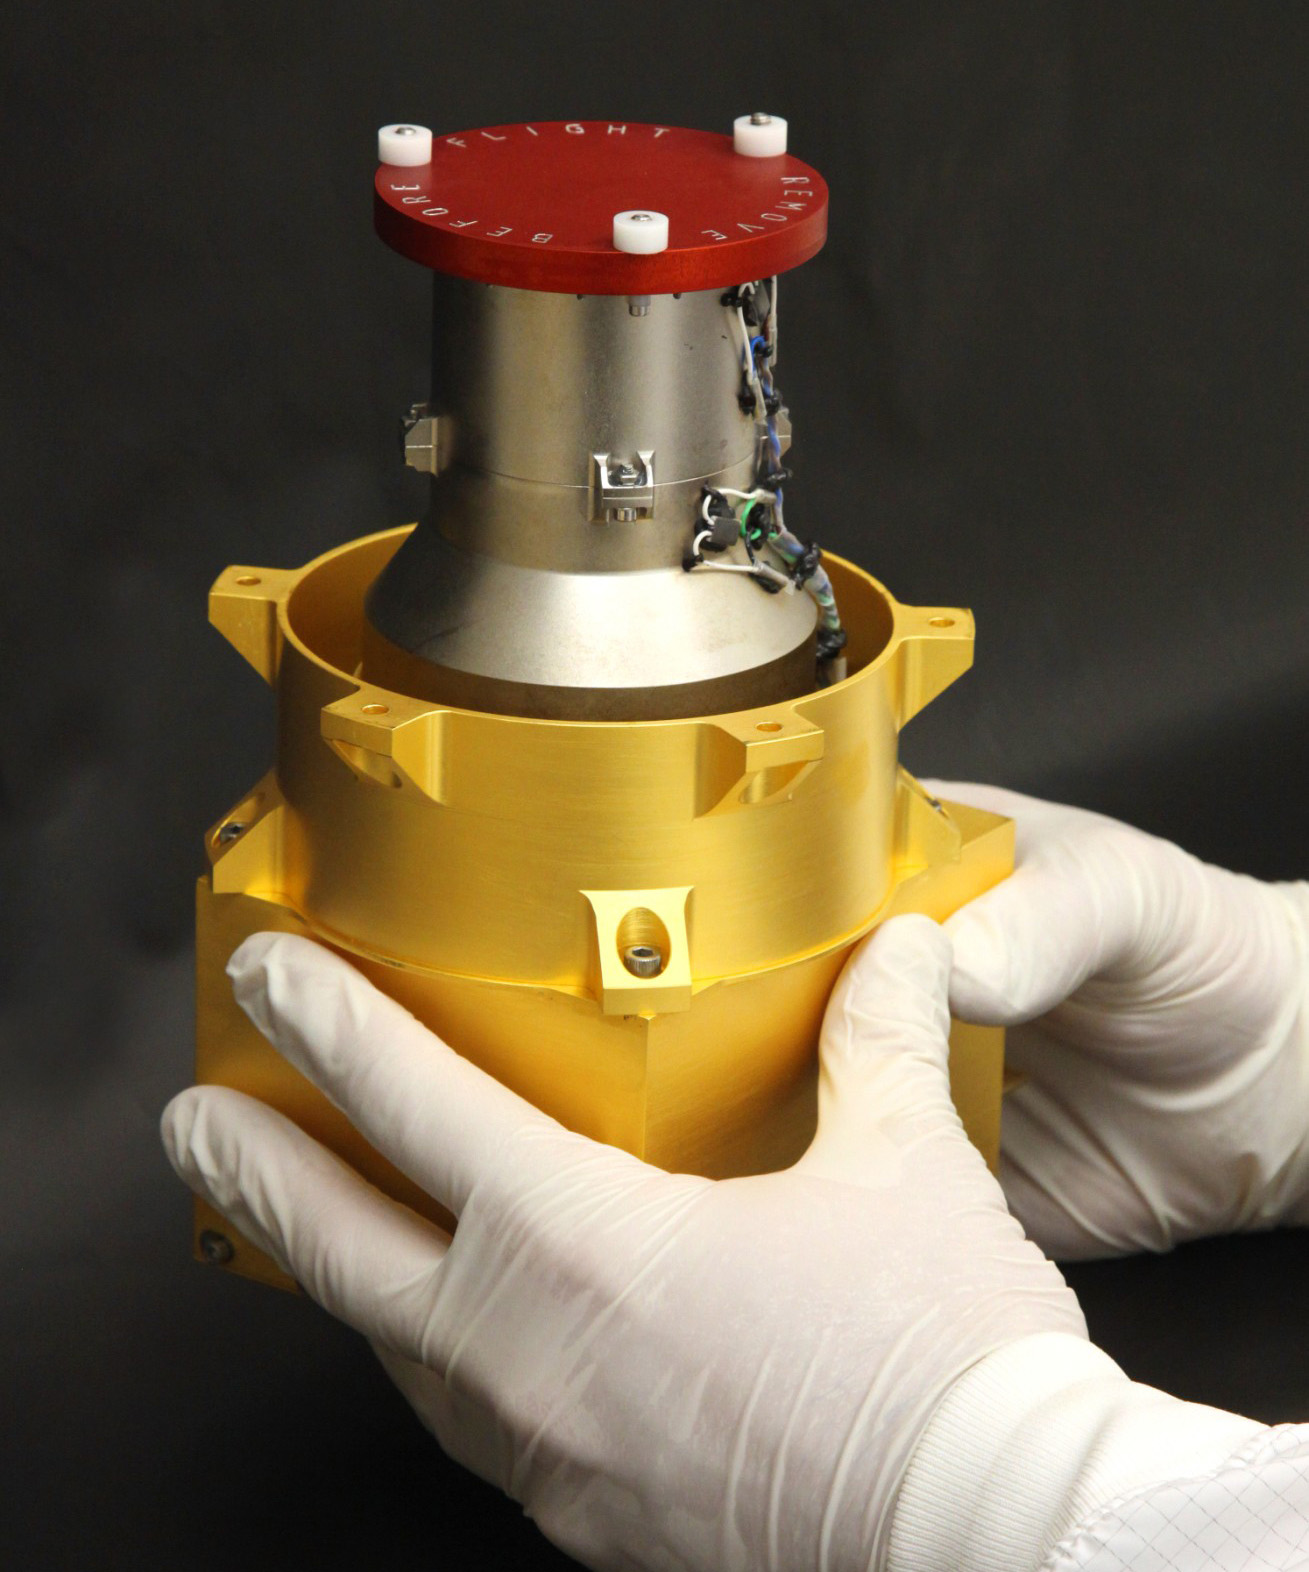
\includegraphics[scale=.10]{figures/fig6_2.jpg}
			%\caption{Spettri energetici di diversi ioni nei GCR \cite{saggiatore}}
		\end{figure}
		\begin{block}{}
		RAD: calorimetro $CsI$ per particelle cariche e raggi $\gamma$
		\end{block}
    \end{column}
\end{columns}
\end{frame}



%==================================================================
						%SLIDE - Schermature
%==================================================================

\section{Schermature}
\begin{frame} [fragile]
	\frametitle{Schermature}
	\small
	
Esistono tre mezzi per ridurre l'esposizione alle radiazioni ionizzanti:
\begin{itemize}
\item \colorbox{yellow}{Aumentare la distanza} dalla sorgente di radiazione $\Longrightarrow$ GCR \textcolor{red}{isotropo}
\item \colorbox{yellow}{Ridurre il tempo} di esposizione $\Longrightarrow$ \textcolor{red}{in aumento} secondo i piani di esplorazione e colonizzazione
\item \colorbox{yellow}{Schermare} la radiazione $\Longrightarrow$ Sfortunatamente, la schermatura nello spazio \`e problematica
\end{itemize}


Quando colpiscono gli scudi le radiazioni cosmiche producono particelle secondarie e neutroni mediante frammentazione nucleare.
\newline

Sia la perdita di energia (formula di Bethe-Bloch $-\frac{<dE>}{dx}$ $\sim$ $Z$$/$$A$) \newline
sia le sezioni d'urto di frammentazione nucleare per unit\`a di massa (formula di Bradt-Peters $\sigma$ $\sim$ $A^{-1/3}$) diminuiscono aumentando il numero atomico $A$. 
\begin{block}{}
I materiali leggeri e altamente idrogenati sono di pi\`u efficaci nel ridurre la dose rispetto a materiali pesanti ad alto $Z$ come $Al$ (materiale strutturale comune nel veicolo spaziale) o $Pb$.
\end{block}
Approfondimenti: \textcolor{blue}{\textit{Space radiation protection: Destination Mars - Marco Durante}}
\end{frame}



%==================================================================
						%SLIDE - Schermature
%==================================================================

\begin{frame} [fragile]
	\frametitle{Schermature}
	\begin{figure}
	  \centering
			\includegraphics[scale=.040]{figures/fig6.jpg}
			\caption{Artist's view of the mars ice house. Image from the NASA image gallery}
		\end{figure}
\colorbox{pink}{$H_{2}O$  materiale schermante efficace}, un'opzione interessante sarebbe quella di \colorbox{yellow}{coprire una base gonfiabile con un guscio di ghiaccio}, che potrebbe essere estratto da Marte. La casa di ghiaccio di Marte sarebbe quasi trasparente, permettendo cos\`i alla luce naturale di entrare.
\end{frame}

%==================================================================
						%SLIDE - Schermature
%==================================================================

\begin{frame} [fragile]
	\frametitle{Schermature}
	\begin{figure}
	  \centering
			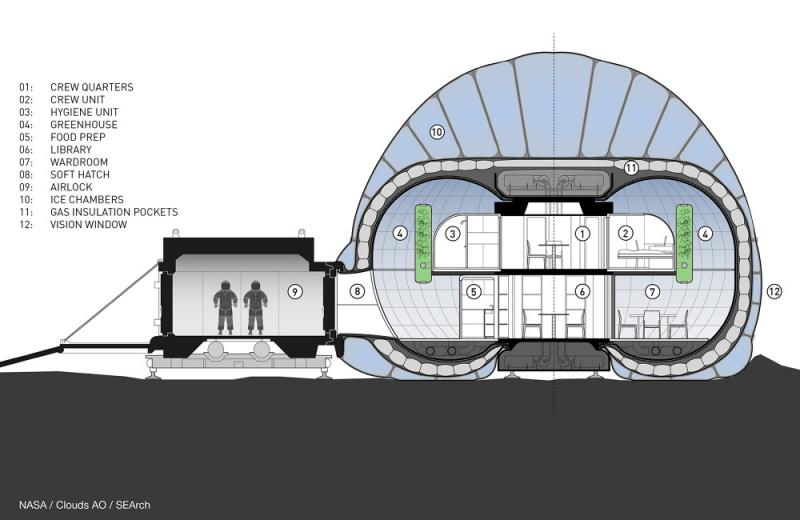
\includegraphics[scale=.30]{figures/fig4.jpg}
			%\caption{$\varphi$ angolo azimutale, $\vartheta$ angolo polare}
			%\begin{tikzpicture}
            		%\node[anchor=south west,inner sep=0] at (0,0) {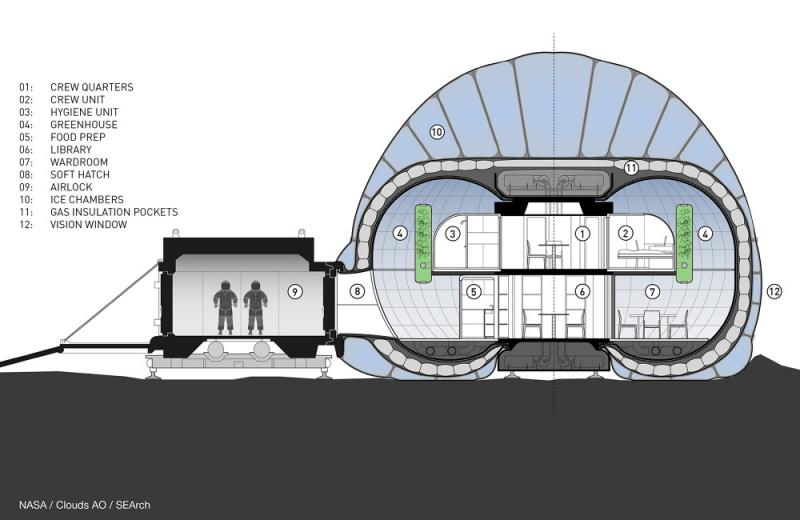
\includegraphics[width=1\textheight]{figures/fig4}};
            		%\draw<1>[red,ultra thick,rounded corners] (1.5,3) rectangle (0, 4);
        			%\end{tikzpicture}
		\end{figure}
Questo \textbf{risultato paradossale} \`e causato dalla \textcolor{blue}{generazione di neutroni}, il cui fattore di alta qualita' alla fine aumenta la dose equivalente dietro lo scudo. Tutti i codici suggeriscono che \textcolor{red}{non vi sar\`a alcun guadagno nei rifugi pi\`u pesanti}.
\end{frame}


%==================================================================
						%SLIDE - thebibliography
%==================================================================

\begin{frame}
\frametitle{\refname}
   \begin{thebibliography}{9}
   \small
   

      \bibitem{BLANCATO} Antonella Alessandra Blancato
      \newblock \textit{Rischi da radiazione nei voli interplanetari}
      \newblock \emph{Tesi di Laurea}, 2007-2008
      
      \bibitem{saggiatore} Marco Durante
      \newblock \textit{Recent advances in space Radiation Protection}
      \newblock \emph{Il Nuovo Saggiatore Vol 33}, 2017
      
      \bibitem{Nasa1} Nasa
      \newblock \textit{Nasa Space Radiation Ebook}
      \newblock \emph{https://www.nasa.gov/hrp/elements/radiation} 2020.
      
      \bibitem{Nasa2} Nasa, CERN
      \newblock \textit{NASA, CERN Timepix Technology Advances Miniaturized Radiation Detection}
      \newblock \emph{https://www.nasa.gov/hrp/elements/radiation} 2020.

      \bibitem{Rad} Vincenzo Patera - Rome University ?La Sapienza?
      \newblock \textit{Radioprotection In Space}
      %\newblock \emph{http://arpg-serv.ing2.uniroma1.it/patera/didattica/FisRadMed/Lezione_RadioprotectionSpace} 

      
   \end{thebibliography}
\end{frame}
%==================================================================

\end{document}